% !TeX spellcheck = pt_BR
%%\documentclass[]{scrartcl}
\documentclass[a4paper, oneside]{article}

%% Language and font encodings
\usepackage[portuguese]{babel}
\usepackage[utf8x]{inputenc}
\usepackage[T1]{fontenc}

%% Sets page size and margins
\usepackage[a4paper,top=2.2cm,bottom=2.2cm,left=2cm,right=2cm,marginparwidth=1.75cm]{geometry}

%% Useful packages
\usepackage{amsmath}
\usepackage{graphicx}


\usepackage{fancyhdr}
\usepackage{titlepic}
\usepackage{tabto}
\usepackage{amsfonts}
\usepackage{commath}
\usepackage{float}
\usepackage{setspace}
\usepackage[labelfont=bf]{caption}
\usepackage{subcaption}
\usepackage[table,xcdraw]{xcolor}
\usepackage{subfiles}
\usepackage{multicol}
\usepackage{comment}
\usepackage{color}
\usepackage{mathtools}
%\usepackage[dvipsnames]{xcolor}
\usepackage{lastpage}
\usepackage{indentfirst}
\usepackage{titlesec}
\usepackage{siunitx}
\usepackage{multirow}
\usepackage{enumitem}
\usepackage{textcomp}
\usepackage{gensymb}
\usepackage{systeme}
\usepackage{wrapfig}
\usepackage[numbered,framed]{matlab-prettifier}
\usepackage{hyperref}

\let\ph\mlplaceholder % shorter macro
\lstMakeShortInline"

\lstset{
	style              = Matlab-editor,
	basicstyle         = \mlttfamily,
	escapechar         = ",
	mlshowsectionrules = true,
}

\titleformat{\paragraph}
{\normalfont\normalsize\bfseries}{\theparagraph}{1em}{}
\titlespacing*{\paragraph}
{0pt}{3.25ex plus 1ex minus .2ex}{1.5ex plus .2ex}

\renewcommand{\baselinestretch}{1.2}

%\hypersetup{colorlinks,citecolor=black,filecolor=black,linkcolor=black,urlcolor=black} 

\pagestyle{fancy}
\fancyhf{}
\cfoot{Página  \thepage \hspace{1pt} de \pageref{LastPage}}


%opening
\title{EGer Lab 1}
\author{L. Pedroso}
\begin{document}

\maketitle

\section{Estudo funcional do conversor D/A}
\subsection{Trabalho experimental}
A montagem da Fig. \ref{fig:esquema_DAC} foi executada  no módulo experimental TEE-08, apresentado na Fig. \ref{sec:modulo_experimental}, em que as entradas $S_1,\ldots,S_4$ do DAC são fornecidas diretamente das quatro portas lógicas NOR. O valor da resistência $R_f$ foi ajustado para $R_f = 2R$, numa primeira instância, e $R_f = 4R$ seguidamente. Na Fig.\ref{fig:DAC_exp} são apresentadas as formas de onda observadas em laboratório para os dois valores selecionados para $R_f$. Analisando estas formas de onda verifica-se que a sua forma é muito semelhante ao esperado teoricamente, apresentado graficamente na Fig. \ref{fig:contador_tensao}. Na verdade, é de salientar que as escalas das Figs.  \ref{fig:2R_DAC_exp} e \ref{fig:4R_DAC_exp} foram propositadamente ajustadas por forma a serem iguais, sendo visível que a diferença de tensão entre patamares é o sensivelmente o dobro para $R_f = 4R$ em relação a $R_f = 2R$, como previsto na Secção \ref{sec:DAC_teor}. É também visível que, a transição do patamar de maior tensão para o patamar de menor tensão não é instantânea. Este fenómeno é devido ao \textit{slew rate} do AmpOp e será estudado com mais detalhe na Secção \ref{sec:slewRate}.

\begin{figure}[ht]
	\centering
	\begin{subfigure}[b]{0.5\textwidth}
		\centering
		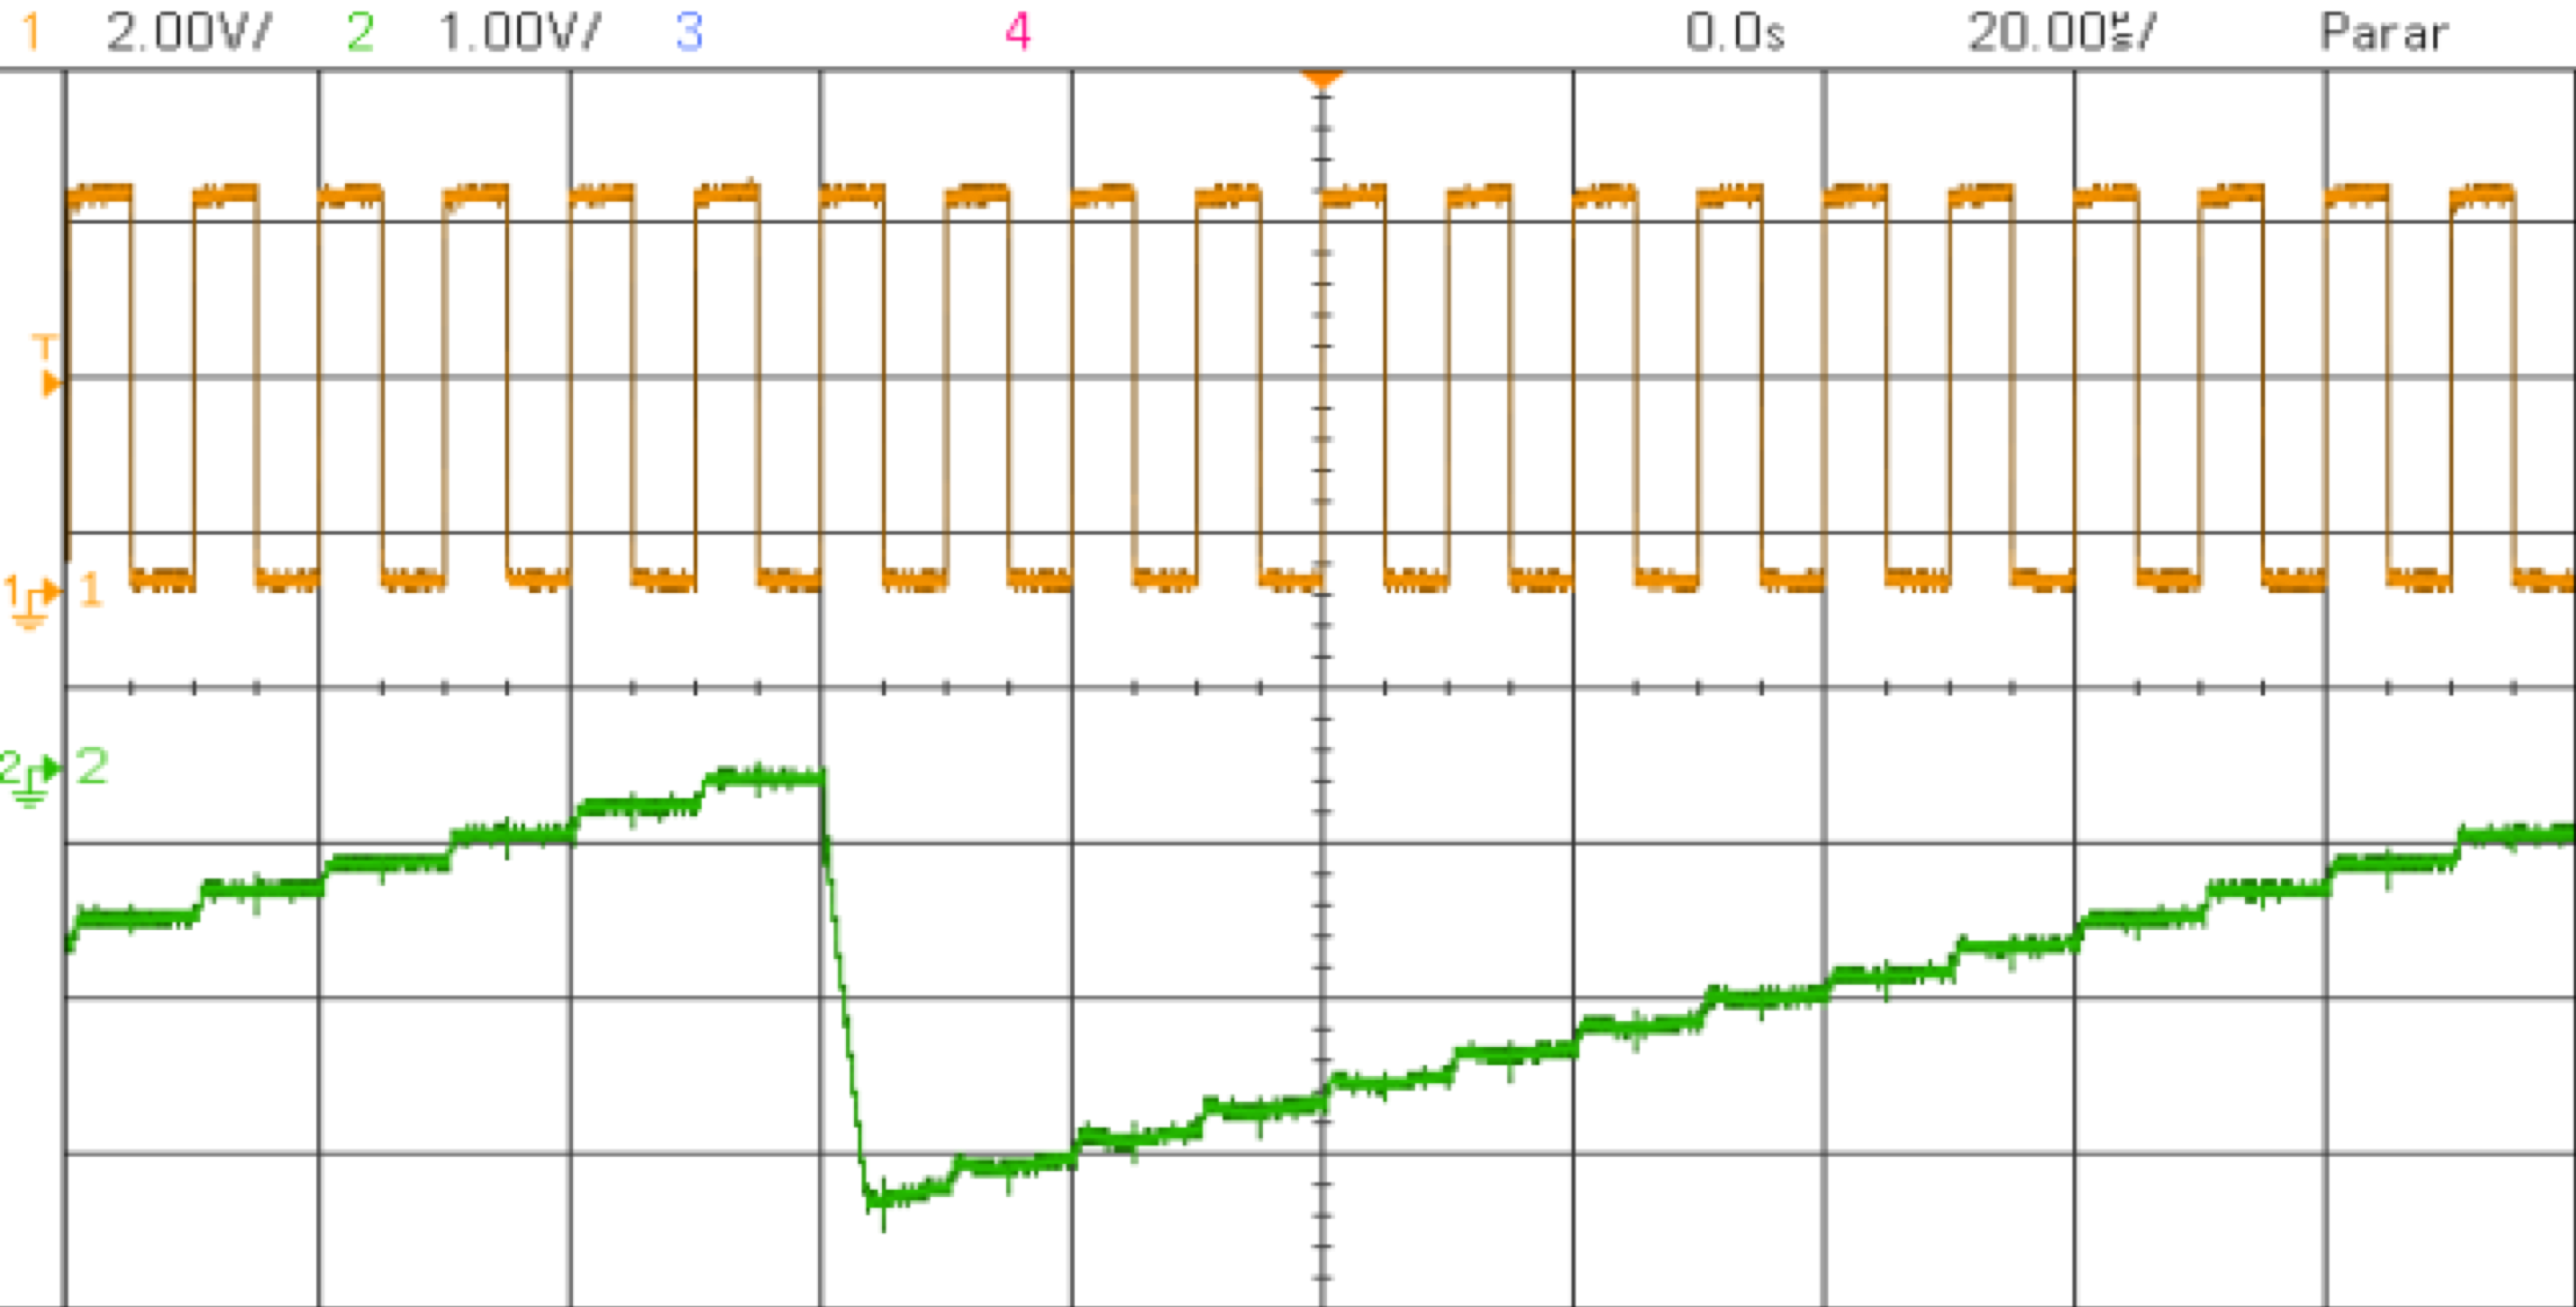
\includegraphics[width=\textwidth]{figures/2R_DAC_exp.png}
		\caption{$R_f=2R$.\\}
		\label{fig:2R_DAC_exp}
	\end{subfigure}%
	\hfill
	\begin{subfigure}[b]{0.5\textwidth}
		\centering
		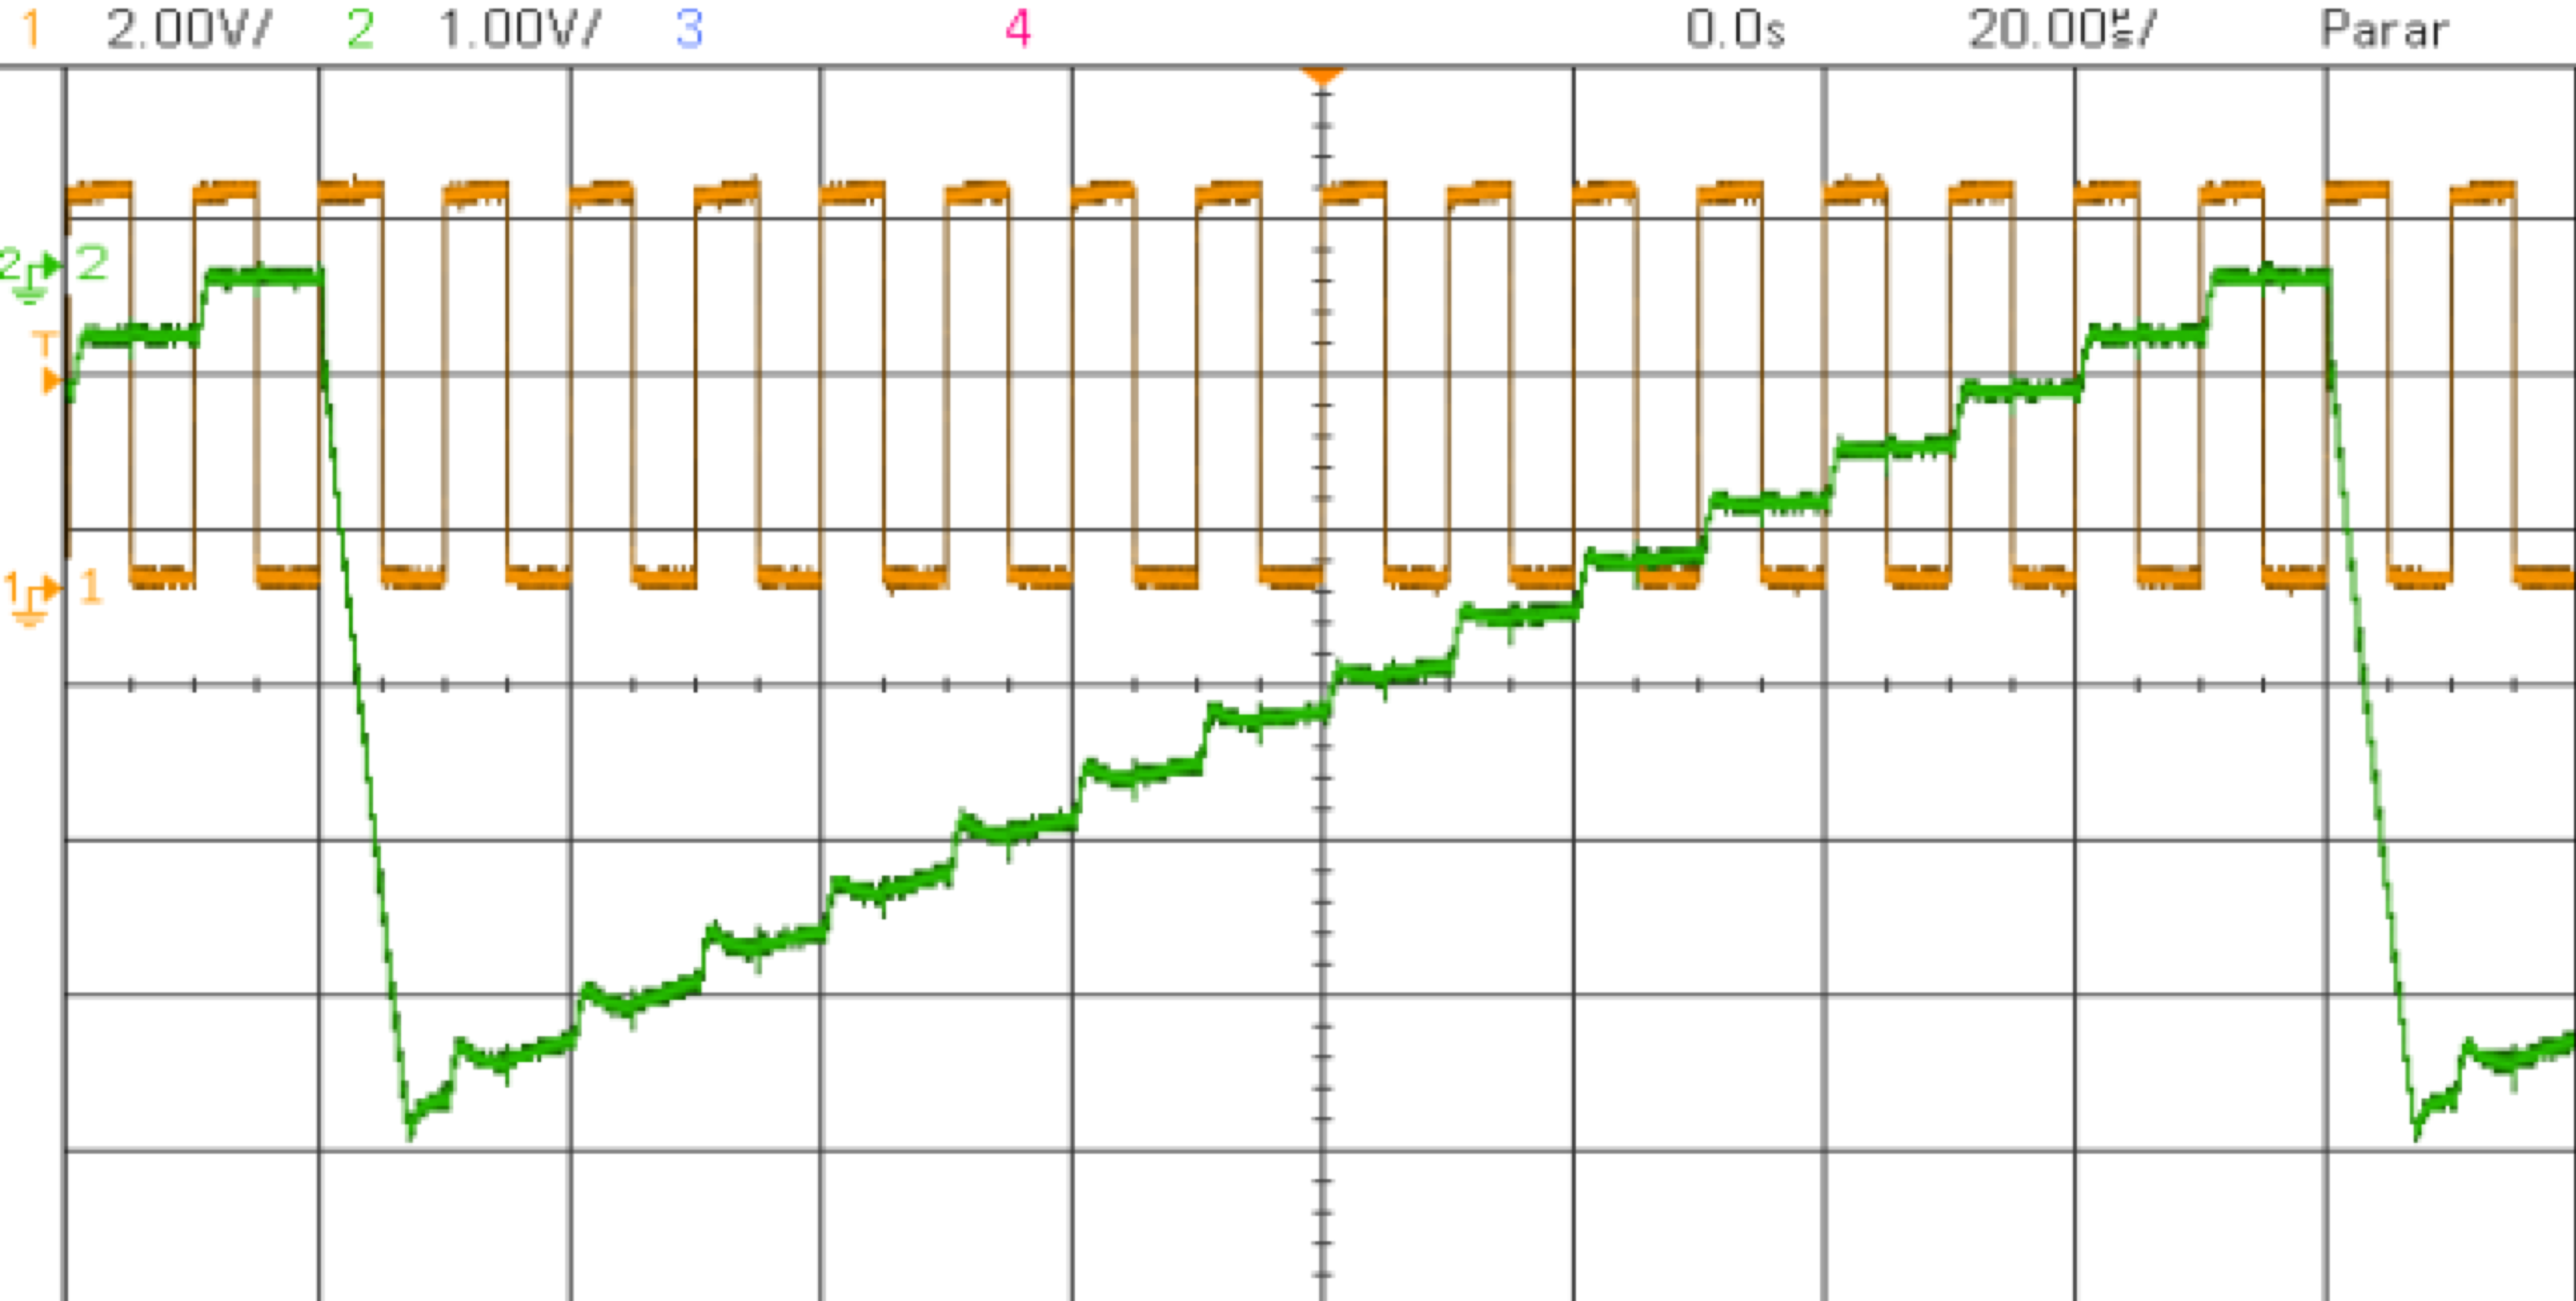
\includegraphics[width=\textwidth]{figures/4R_DAC_exp.png}
		\caption{$R_f=4R$.\\}
		\label{fig:4R_DAC_exp}
	\end{subfigure}%
	\caption{Sinais observados no osciloscópio da saída do DAC (verde) e do sinal de \textit{clock} (laranja).\\}
	\label{fig:DAC_exp}
\end{figure}
 
\subsection{Comparação de resultados}\label{sec:cmpEstudoFunc}

Nesta subsecção os resultados experimentais obtidos em laboratório, e apresentados na subsecção anterior, são analisados com detalhe e comparados com os previstos teoricamente na Secção \ref{sec:DAC_teor}. Na Fig. \ref{fig:DAC_exp_cmp} são apresentados os sinais observados nos osciloscópio no laboratório com os previstos teoricamente, para 16 períodos de \textit{clock}, tanto para $R_f = 2R$ como para $R_f = 4R$. Foi omitida a transição $15\rightarrow 0$, visto que ela será estudada detalhadamente na Secção \ref{sec:slewRate}. Ao analisar estas figuras, comparando os valores experimentais com os teóricos é evidente a existência de um grande desfasamento entre eles. Na verdade, verificamos que a componente principal do desfazamento verificado é proporcional à tensão de saída do DAC, não existindo uma componente de erro não proporcional que seja significativa. Este fenómeno verifica-se para ambos os valores de $R_f$ usados. Assim, analisando a equação que expressa a saída do DAC \eqref{eq:DAC_output} podemos concluir que a existência de um erro proporcional predominante é indicativo que a fonte de erro predominante é: i) a resistência $R_f$; ii) a tensão lógica $V_{ref}$; ou iii) a combinação de i) e ii).

\begin{figure}[ht]
	\centering
	\begin{subfigure}[b]{0.5\textwidth}
		\centering
		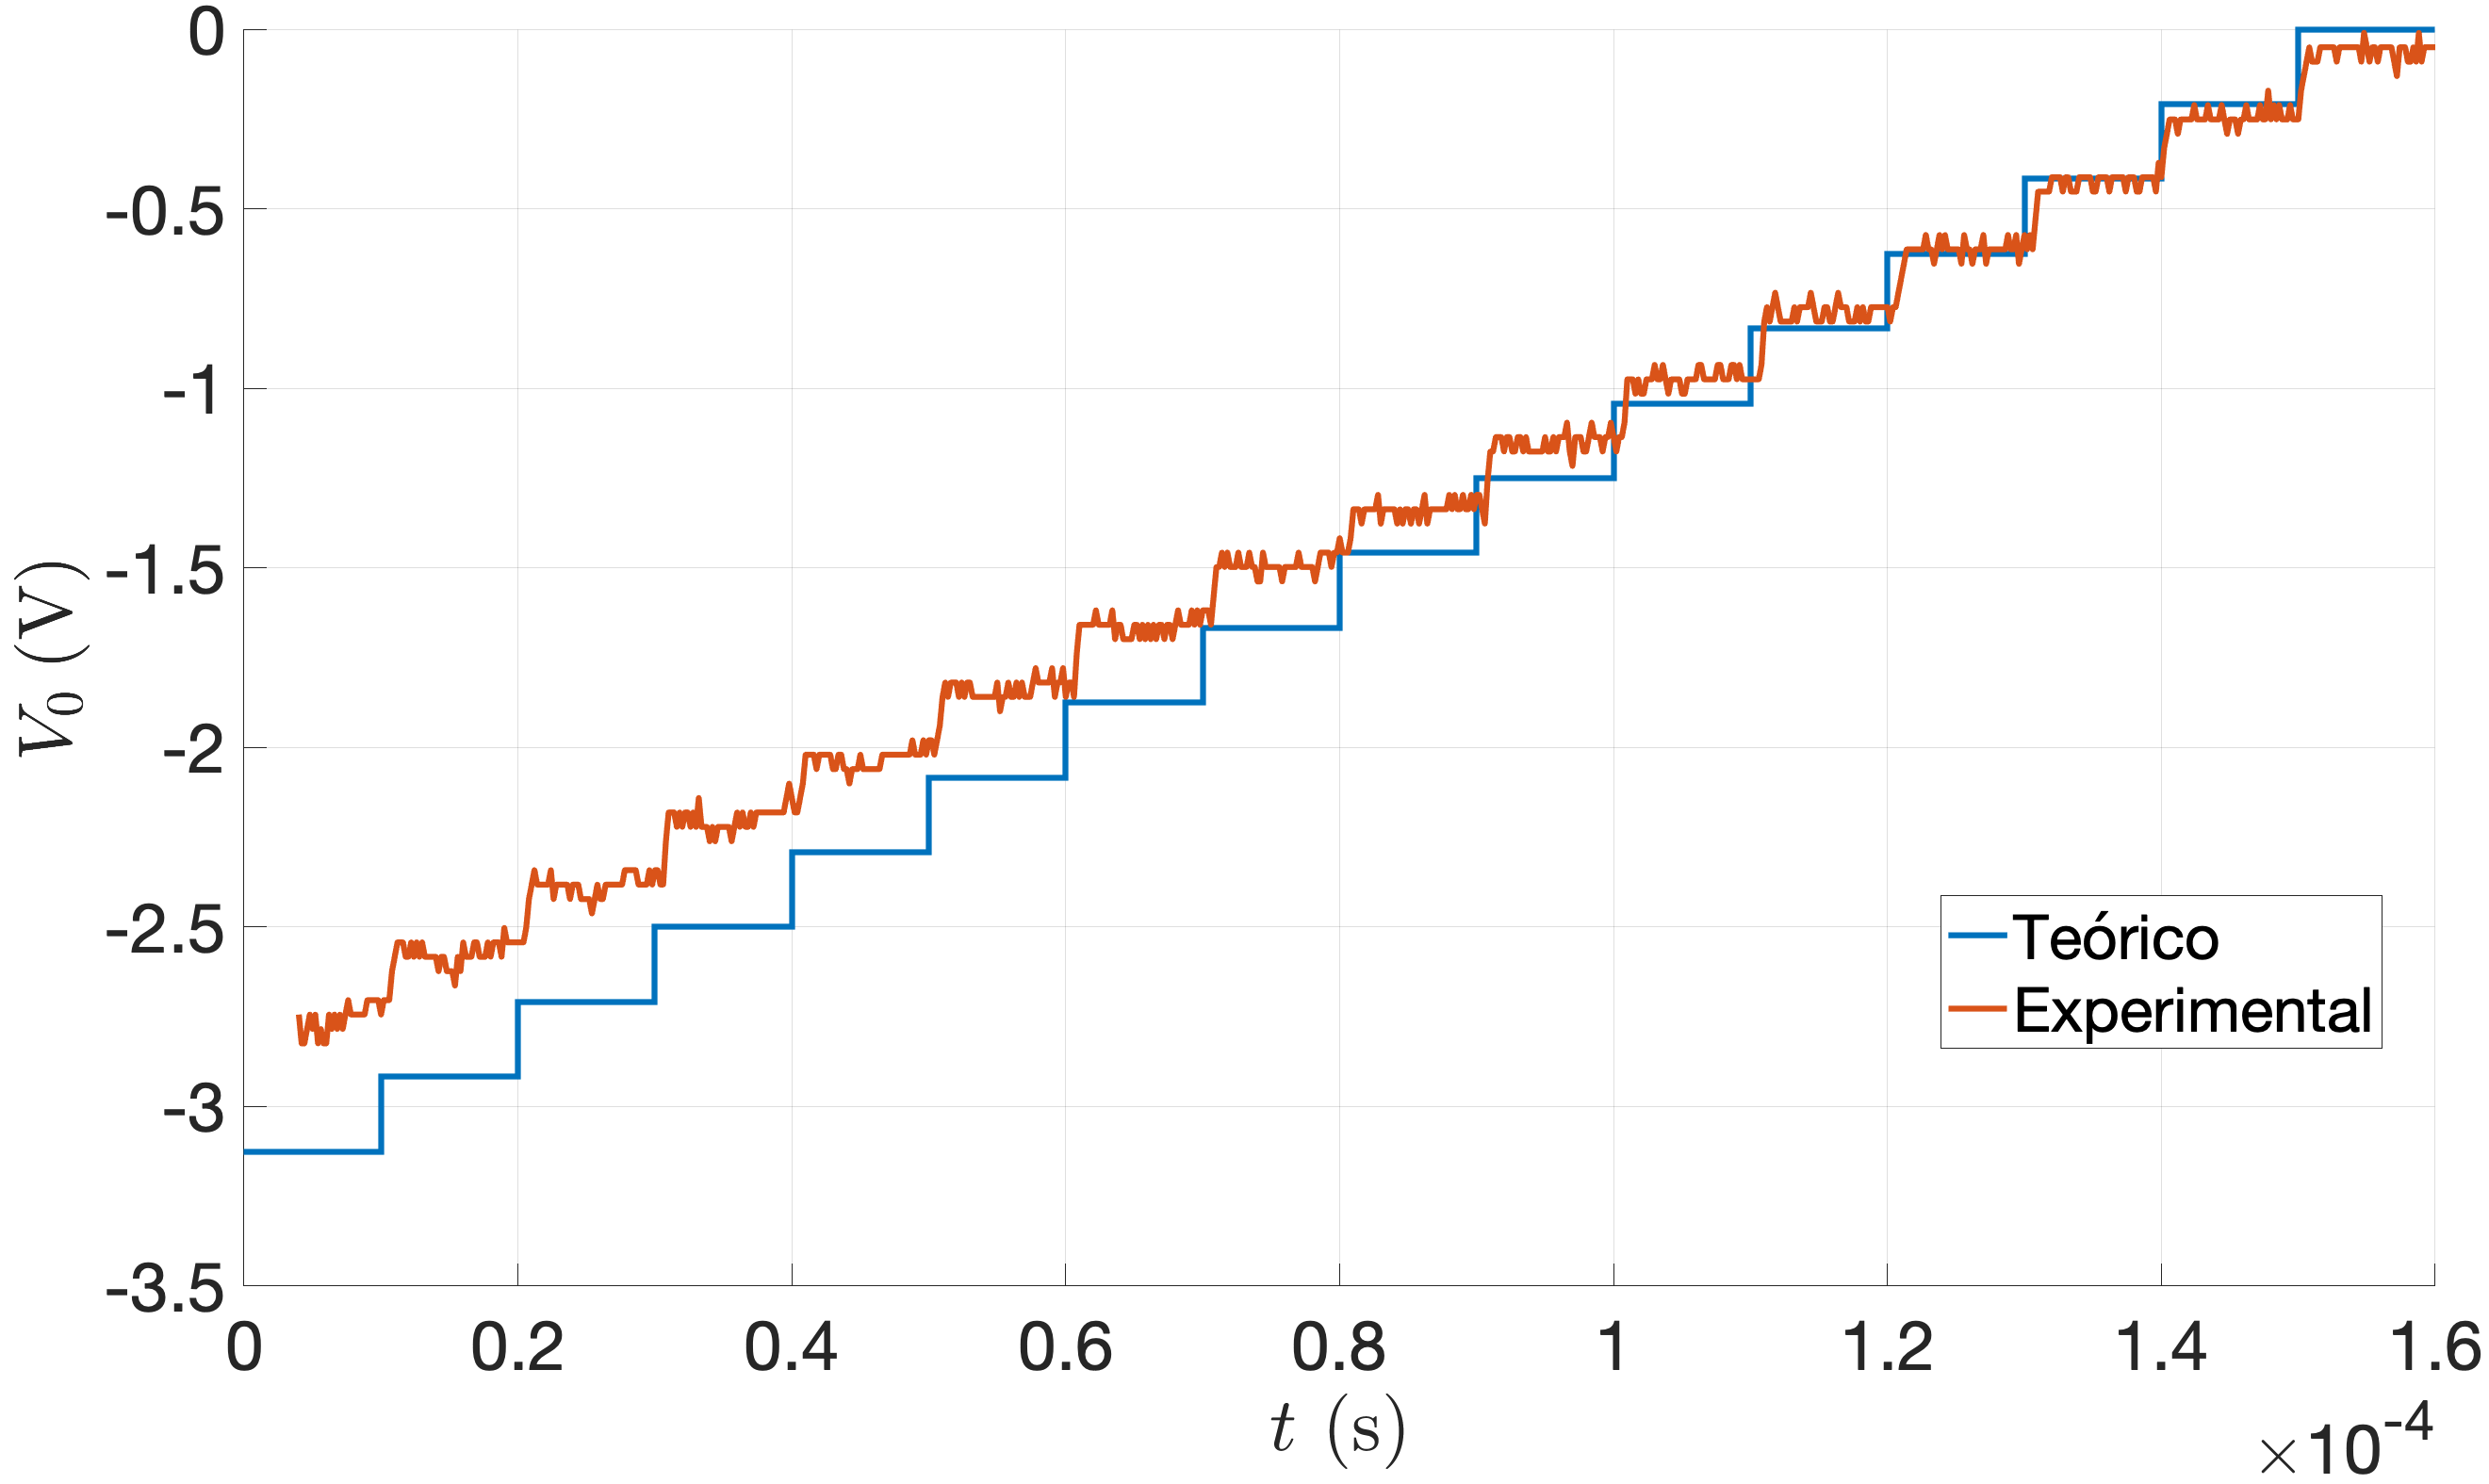
\includegraphics[width=\textwidth]{figures/4_3_2_DAC_2R.png}
		\caption{$R_f=2R$.\\}
		\label{fig:4_3_2_DAC_2R}
	\end{subfigure}%
	\hfill
	\begin{subfigure}[b]{0.5\textwidth}
		\centering
		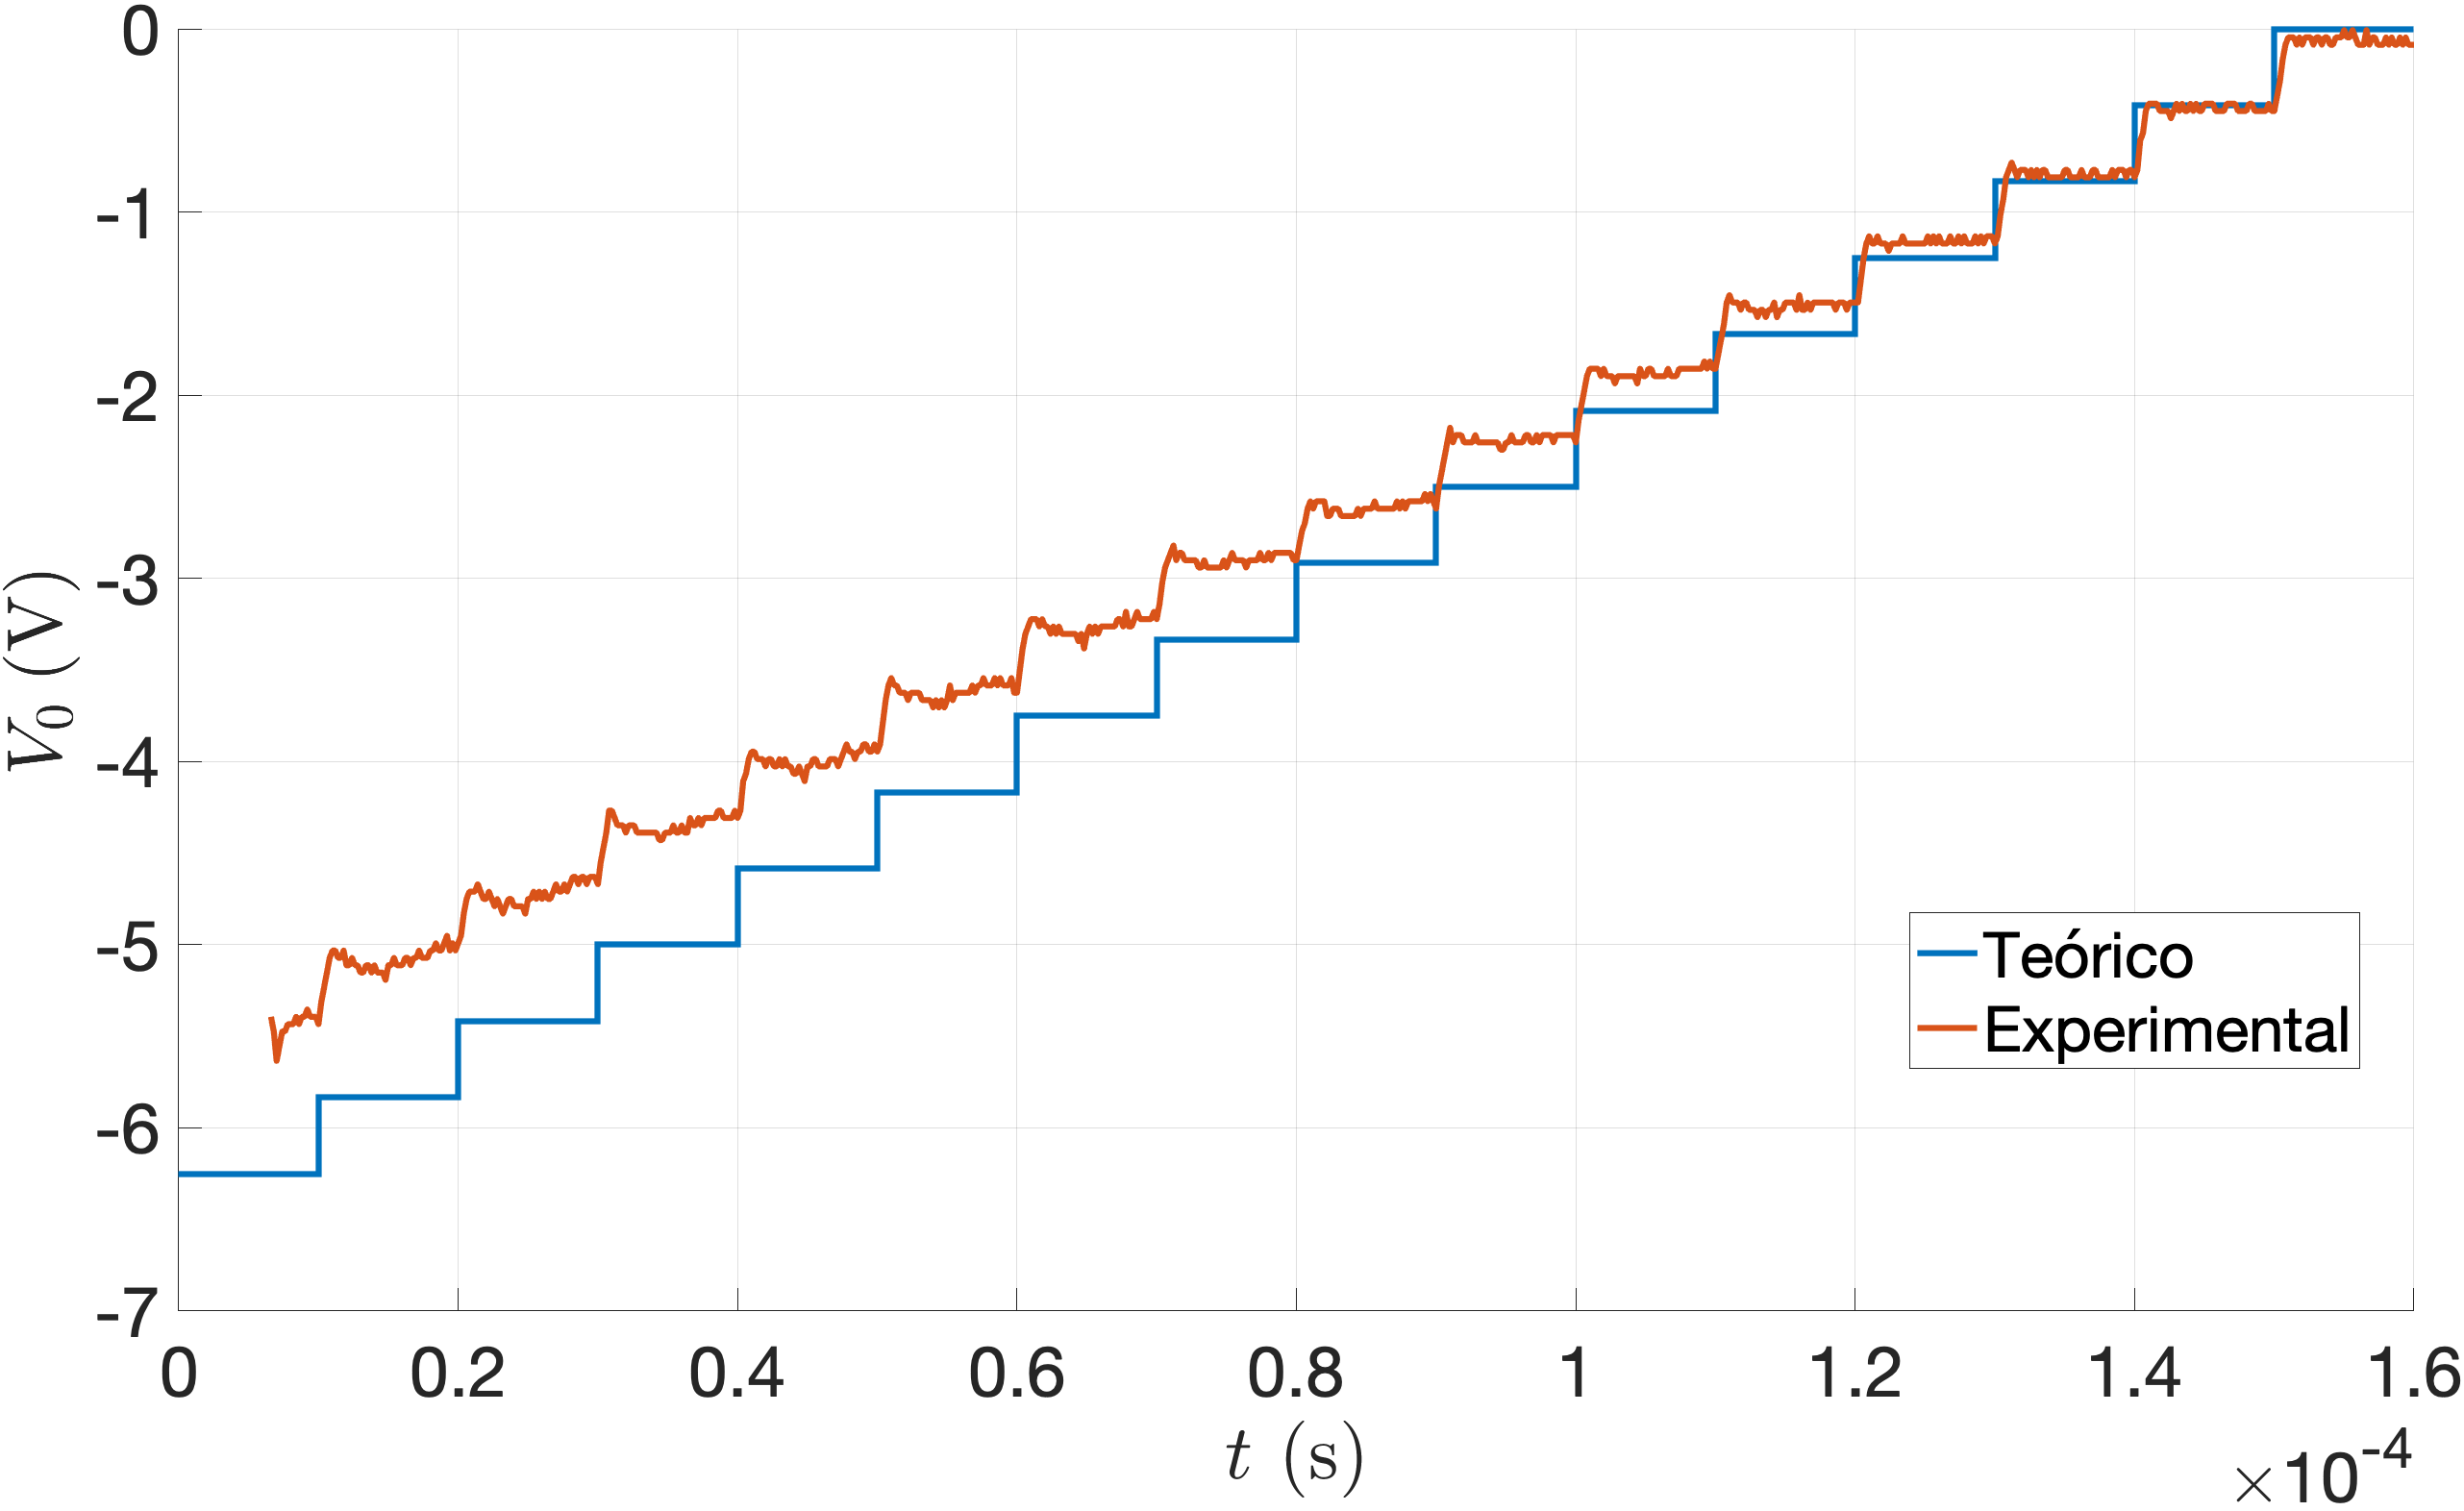
\includegraphics[width=\textwidth]{figures/4_3_2_DAC_4R.png}
		\caption{$R_f=4R$.\\}
		\label{fig:4_3_2_DAC_4R}
	\end{subfigure}%
	\caption{Comparação dos sinais observados no osciloscópio da saída do DAC com os esperados teoricamente, ao longo de 16 períodos de \textit{clock}.\\}
	\label{fig:DAC_exp_cmp}
\end{figure}

Por forma avaliar com mais detalhe e objetivamente o desfasamento entre resultados teóricos e experimentais, determinou-se o valor dos patamares de tensão experimentais correspondendo a cada um dos números representados em binário à saída das portas lógicas NOR. Para tal, o sinal obtido do osciloscópio foi filtrado fazendo uso de um filtro \textit{moving average} com uma janela de retrocesso de 10 amostras e de avanço de 9 amostras (com um total de $10+1+9 = 20$ amostras). A tensão do patamar foi estimada como sendo o valor de tensão do sinal filtrado aquando da queda do sinal de \textit{clock}, \textit{i.e.}, a meio de cada patamar. Os valores de tensão de cada patamar obtidos experimentalmente, bem como a sua comparação com o respetivos valores previstos teoricamente, são apresentados nas Tabelas \ref{tab:Pat2R_exp} e \ref{tab:Pat4R_exp}, respetivamente para $R_f = 2R$ e $R_f = 4R$. Como observado na análise das formas de onda obtidas no laboratório verificamos que para $Q = 0,\ldots,7$, para ambos os valores de $R_f$, o desfazamento relativo é aproximadamente constante, indicando a presença de erro proporcional com a tensão. Para valores de $Q>7$ a tensão $V_0$ é mais reduzida em módulo, portanto a componente proporcional do erro deixa de ser preponderante, e outras componentes do erro associadas ao método experimental começam a fazer-se notar, como por exemplo, desfazamentos nos valores das resistências da escada R-2R e o erro de quantização do osciloscópio. É de salientar que o elevado erro relativo visível para $Q=14$ e $R_f = 2R$ é causados pelo facto de se estar a trabalhar mais reduzidas, e a exatidão das medições nesta situação se degradar. A degradação da exatidão é devida ao baixo rácio sinal-ruído (SNR) num sinal próximo de 0.  Ainda que o erro relativo seja significativo, o erro absoluto é inferior a um quinto da separação teórica entre patamares. Na Tabela \ref{tab:Pat4R_exp} é ainda apresentado o rácio entre patamares com o mesmo $Q$ para $R_f = 4R$ e $R_f = 2R$. Verificamos que o quociente de todos os valores são muito próximos do valor esperado teoricamente de 2, como analisado na Secção \ref{sec:DAC_teor}. Note-se que não faz sentido calcular o rácio para $Q=15$ visto que se prevê que a saída do DAC seja nula em ambas as situações. De facto, ainda que experimentalmente não seja nula, são muito reduzidas em módulo, pelo que o valor resultante não faria sentido, dada o baixo SNR da amostragem.

\begin{table}[ht]
	\centering
	\caption{Comparação entre a tensão dos patamares medida experimentalmente e esperada teoricamente para $R_f = 2R$.}
	\label{tab:Pat2R_exp}
	\begin{tabular}{ccccc}
		$Q$ & Teórico (V) & Experimental (V) & Erro absoluto (V) & Erro relativo\\
		\hline
		0 & -3.125 & -2.784 & 0.3410 & 10.91\%\\ 
		1 & -2.917 & -2.591 & 0.3256 & 11.17\%\\
		2 & -2.708 & -2.402 & 0.3063 & 11.31\%\\ 
		3 & -2.500 & -2.219 & 0.2808 & 11.23\%\\ 
		4 & -2.292 & -2.052 & 0.2393 & 10.44\%\\ 
		5 & -2.083 & -1.851 & 0.2320 & 11.14\%\\ 
		6 & -1.875 & -1.674 & 0.2006 & 10.70\%\\ 
		7 & -1.667 & -1.5 & 0.1671 & 10.03\%\\ 
		8 & -1.458 & -1.347 & 0.1115 & 7.648\%\\ 
		9 & -1.250& -1.156 & 0.09416 & 7.533\%\\ 
		10& -1.042 & -0.9729 & 0.06874 & 6.599\%\\ 
		11& -0.8333 & -0.784 & 0.04935 & 5.922\%\\ 
		12& -0.6250 & -0.6131 & 0.01187 & 1.899\%\\ 
		13& -0.4167 & -0.4242 & -0.007517 & -1.804\%\\ 
		14& -0.2083 & -0.2493 & -0.04098 & -19.67\%\\ 
		15& 0.0000 & -0.05433 & -0.05433 & -- \\
		\hline
	\end{tabular}
\end{table}


\begin{table}[ht]
	\centering
	\caption{Comparação entre a tensão dos patamares medida experimentalmente e esperada teoricamente para $R_f = 4R$.}
	\label{tab:Pat4R_exp}
	\begin{tabular}{cccccc}
		$Q$ & Teórico (V) & Experimental (V) & ${V_0}_{4R}/{V_0}_{2R}$ & Erro absoluto (V) & Erro relativo\\
		\hline
		0 & -6.250 & -5.470 & 1.965 & 0.7802 & 12.48\%\\ 
		1 & -5.833 & -5.120 & 1.976 & 0.7132 & 12.23\%\\ 
		2 & -5.417 & -4.762 & 1.983 & 0.6544 & 12.08\%\\ 
		3 & -5.000 & -4.382 & 1.975 & 0.6176 & 12.35\%\\ 
		4 & -4.583 & -4.025 & 1.961 & 0.5587 & 12.19\%\\ 
		5 & -4.167 & -3.649 & 1.971 & 0.5179 & 12.43\%\\ 
		6 & -3.750 & -3.293 & 1.967 & 0.4570 & 12.19\%\\ 
		7 & -3.333 & -2.919 & 1.947 & 0.4142 & 12.43\%\\ 
		8 & -2.917 & -2.632 & 1.954 & 0.2850 & 9.772\%\\ 
		9 & -2.500 & -2.256 & 1.952 & 0.2442 & 9.769\%\\ 
		10 & -2.083 & -1.890 & 1.943 & 0.1934 & 9.282\%\\ 
		11 & -1.667 & -1.524 & 1.944 & 0.1425 & 8.553\%\\ 
		12 & -1.250 & -1.162 & 1.896 & 0.08769 & 7.015\%\\ 
		13 & -0.8333 & -0.7985 & 1.882 & 0.03484 & 4.181\%\\ 
		14 & -0.4167 & -0.4286 & 1.719 & -0.01198 & -2.874\%\\ 
		15 & 0.0000 & -0.05477 & -- & -0.05477 & --  \\
		\hline
	\end{tabular}
\end{table}

Foi analisada ainda a diferença experimental entre a tensão de patamares consecutivos. Estes valores, bem como a sua comparação com o previsto teoricamente, são apresentados na Tabela \ref{tab:difPat_exp}. Como se verifica a partir da análise desta tabela, os erros relativos são significativos e a diferença entre patamares medida experimentalmente é consistentemente inferior à prevista teoricamente. Este efeito é compatível com a análise anterior da introdução de erro experimental significativo no valor de $V_{ref}$ e $R_f$.

\begin{table}[ht]
	\centering
	\caption{Comparação entre diferença entre a tensão em patamares consecutivos medida experimentalmente e esperada teoricamente.}
	\label{tab:difPat_exp}
	\begin{tabular}{ccccc}
		Transição & $\Delta$pat.(V) ($\!R_f\!=\!2R$) & Erro relativo ($\!R_f\!=\!2R$)& $\Delta$pat.(V) ($\!R_f\!=\!4R$) & Erro relativo ($\!R_f\!=\!4R$)\\
		\hline
		$0\rightarrow1$  & 0.1930 & -7.377\% & 0.3497 & 16.06 \%\\ 
		$1\rightarrow2$   & 0.1889 & -9.307\% & 0.3578 & 14.13\%\\ 
		$2\rightarrow3$   & 0.1829 & -12.20\% & 0.3799 & 8.824\%\\ 
		$3\rightarrow4$   & 0.1668 & -19.92\% & 0.3578 & 14.13\%\\ 
		$4\rightarrow5$   & 0.2010 & -3.518\% & 0.3759 & 9.789\%\\ 
		$5\rightarrow6$   & 0.1769 & -15.10\% & 0.3558 & 14.61\%\\ 
		$6\rightarrow7$   & 0.1749 & -16.06\% & 0.3739 & 10.27\%\\ 
		$7\rightarrow8$   & 0.1528 & -26.67\% & 0.2874 & 31.02\%\\ 
		$8\rightarrow9$   & 0.1910 & -8.342\% & 0.3759 & 9.789\%\\ 
		$9\rightarrow10$   & 0.1829 & -12.20\% & 0.3658 & 12.20\%\\ 
		$10\rightarrow11$  & 0.1889 & -9.307\% & 0.3658 & 12.20\%\\ 
		$11\rightarrow12$  & 0.1709 & -17.99\% & 0.3618 & 13.17\%\\ 
		$12\rightarrow13$  & 0.1889 & -9.307\% & 0.3638 & 12.68\%\\ 
		$13\rightarrow14$  & 0.1749 & -16.06\% & 0.3698 & 11.24\%\\ 
		$14\rightarrow15$  & 0.1950 & -6.412\% & 0.3739 & 10.27\%\\
		\hline
	\end{tabular}
\end{table}

Por forma a avaliar se, de facto, é plausível que o desfasamento obtido entre resultados experimentais e resultados previstos teoricamente se deva a desvios dos valores de $V_{ref}$ e $R_f$ experimentais em relação aos seus valores nominais, como analisado anteriormente, iremos calcular os desvios destes parâmetros que explicam os resultados laboratoriais. Seguidamente, usando os valores de $R_f$ e $V_{ref}$ ajustados usando os dados experimentais da Secção \ref{sec:estudoFunc} para calcular resultados teóricos ajustados para o ensaio independente apresentado na Secção \ref{sec:infRes}, será avaliado se estes explicam o observado em laboratório. É de notar que, uma vez que os valores de $V_{ref}$ e $R_f$ são ajustados para explicar os resultados laboratoriais da Secção \ref{sec:estudoFunc}, é evidente que os resultados previstos ajustados para esse ensaio sejam, de forma artificial, muito próximos do observado experimentalmente. No entanto, ao comparar os resultados previsto ajustados com os resultados experimentais para um ensaio distinto e independente (como apresentado na Secção \ref{sec:infRes}) do usado para o ajuste dos parâmetros, é possível avaliar com mais confiança a hipótese feita sobre a origem do erro. Comecemos por assumir, como aproximação, que o erro devido aos desvios de $V_{ref}$ e $R_f$, para tensões à saída do DAC suficientemente elevadas em módulo ($Q<8$), é predominante e que as restantes fontes de erro são desprezáveis. Dada a forma como a montagem é efetuada no módulo experimental TEE-08, apresentado na Fig. \ref{sec:modulo_experimental}, a resistência $R_f$ experimental é dada por $(R_f)_{exp} = (R_a)_{exp}$ para $R_f = 2R$ e $(R_f)_{exp} = (R_a)_{exp}+(R_b)_{exp}$ para $R_f = 4R$. Em que $R_a$ e $R_b$ são resistências presentes no módulo experimental de valor nominal $R_a = R_b=2R$. Destas a única que foi possível medir experimentalmente foi $(R_b)_{exp} = 24.08\text{k}\Omega$. Dividindo a equação da saída do DAC \eqref{eq:DAC_output} usando experimentais pela equação \eqref{eq:DAC_output} usando parâmetros nominais, obtemos a seguinte relação 
\begin{equation}\label{eq:ajusteRf}
\frac{(V_0)_{exp}^{R_f = 2R}(Q = i)}{V_0^{R_f = 2R}(Q = i)} = \frac{(V_{ref})_{exp}}{V_{ref}}\frac{(R_a)_{exp}}{R_a} = \frac{(V_{ref})_{exp}}{V_{ref}}\frac{(R_a)_{exp}}{2R} \:,
\end{equation}
para $R_f = 2R$ e $i = 0, \dots, 7$ e
\begin{equation}\label{eq:ajusteRf2}
\frac{(V_0)_{exp}^{R_f = 4R}(Q = i)}{V_0^{R_f = 4R}(Q = i)} = \frac{(V_{ref})_{exp}}{V_{ref}}\frac{(R_a)_{exp}+(R_b)_{exp}}{R_a+R_b} = \frac{(V_{ref})_{exp}}{V_{ref}}\left(\frac{1}{2}\frac{(R_a)_{exp}}{2R}+\frac{1}{2}\frac{(R_b)_{exp}}{2R}\right)\:,
\end{equation}
para $R_f = 4R$ e $i = 0, \dots, 7$. Temos, da medição de $R_b$, que 
\begin{equation}\label{key}
\frac{(R_b)_{exp}}{2R} = 1.003\:,
\end{equation}
e da média do erro relativo apresentado nas Tabelas \ref{tab:Pat2R_exp} e \ref{tab:Pat4R_exp} para $Q = 0,\ldots,7$ que 
\begin{equation}\label{key}
\frac{(V_0)_{exp}^{R_f = 2R}(Q = i)}{V_0^{R_f = 2R}(Q = i)} = 0.8770 \quad \text{e} \quad \frac{(V_0)_{exp}^{R_f = 2R}(Q = i)}{V_0^{R_f = 2R}(Q = i)} = 0.8913\:.
\end{equation}
Resolvendo \eqref{eq:ajusteRf} e \eqref{eq:ajusteRf2} em ordem a $(R_a)_{exp}/R_a$ e $(V_{ref})_{exp}/V_{ref}$ obtém-se
\begin{equation}\label{key}
(R_a)_{exp}/R_a = 1.020 \quad \text{e} \quad  \frac{(V_{ref})_{exp}}{V_{ref}} = 0.8598\:,
\end{equation}
pelo que $(R_a)_{exp} = 24.48\text{k}\Omega$ e $(V_{ref})_{exp} = 4.299$ V. Assim, para $R_f = 2R$ temos $(R_f)_{exp} = (R_a)_{exp} = 24.48\text{k}\Omega$ e para $R_f = 4R$ temos $(R_f)_{exp} = (R_a)_{exp}+(R_b)_{exp} = 48.56\text{k}\Omega$.

Na Fig. \ref{fig:cteAj_4_3_2_DAC} são apresentados os sinais observados nos osciloscópio no laboratório com os previstos teoricamente com os parâmetros $R_f$ e $V_{ref}$ ajustados, para 16 períodos de \textit{clock}, tanto para $R_f = 2R$ como para $R_f = 4R$. Verificamos que, de facto, os valores previstos teoricamente calculados com os parâmetros ajustados são muito próximos dos observados no laboratório. Este resultado é, no entanto, artificial visto que $R_f$ e $V_{ref}$ foram ajustados para modelar os resultados experimentais obtidos neste ensaio. Por forma a validar, a hipótese de que é plausível que a principal fonte de erro seja $R_f$ e $V_{ref}$, serão comparados os resultados experimentais da Secção \ref{sec:infRes} com os previstos teoricamente com os parâmetros ajustados. É visível, no entanto, que ainda existe uma componente de erro sistemático para $Q>7$, obtendo-se resultados experimentais consistentemente inferiores aos previsão teórica ajustada. Este desfazamento deve-se a desvios em relação aos valores nominais da escada R-2R, que foram desprezados no cálculo de da previsão teórica ajustada.

\begin{figure}[ht]
	\centering
	\begin{subfigure}[b]{0.5\textwidth}
		\centering
		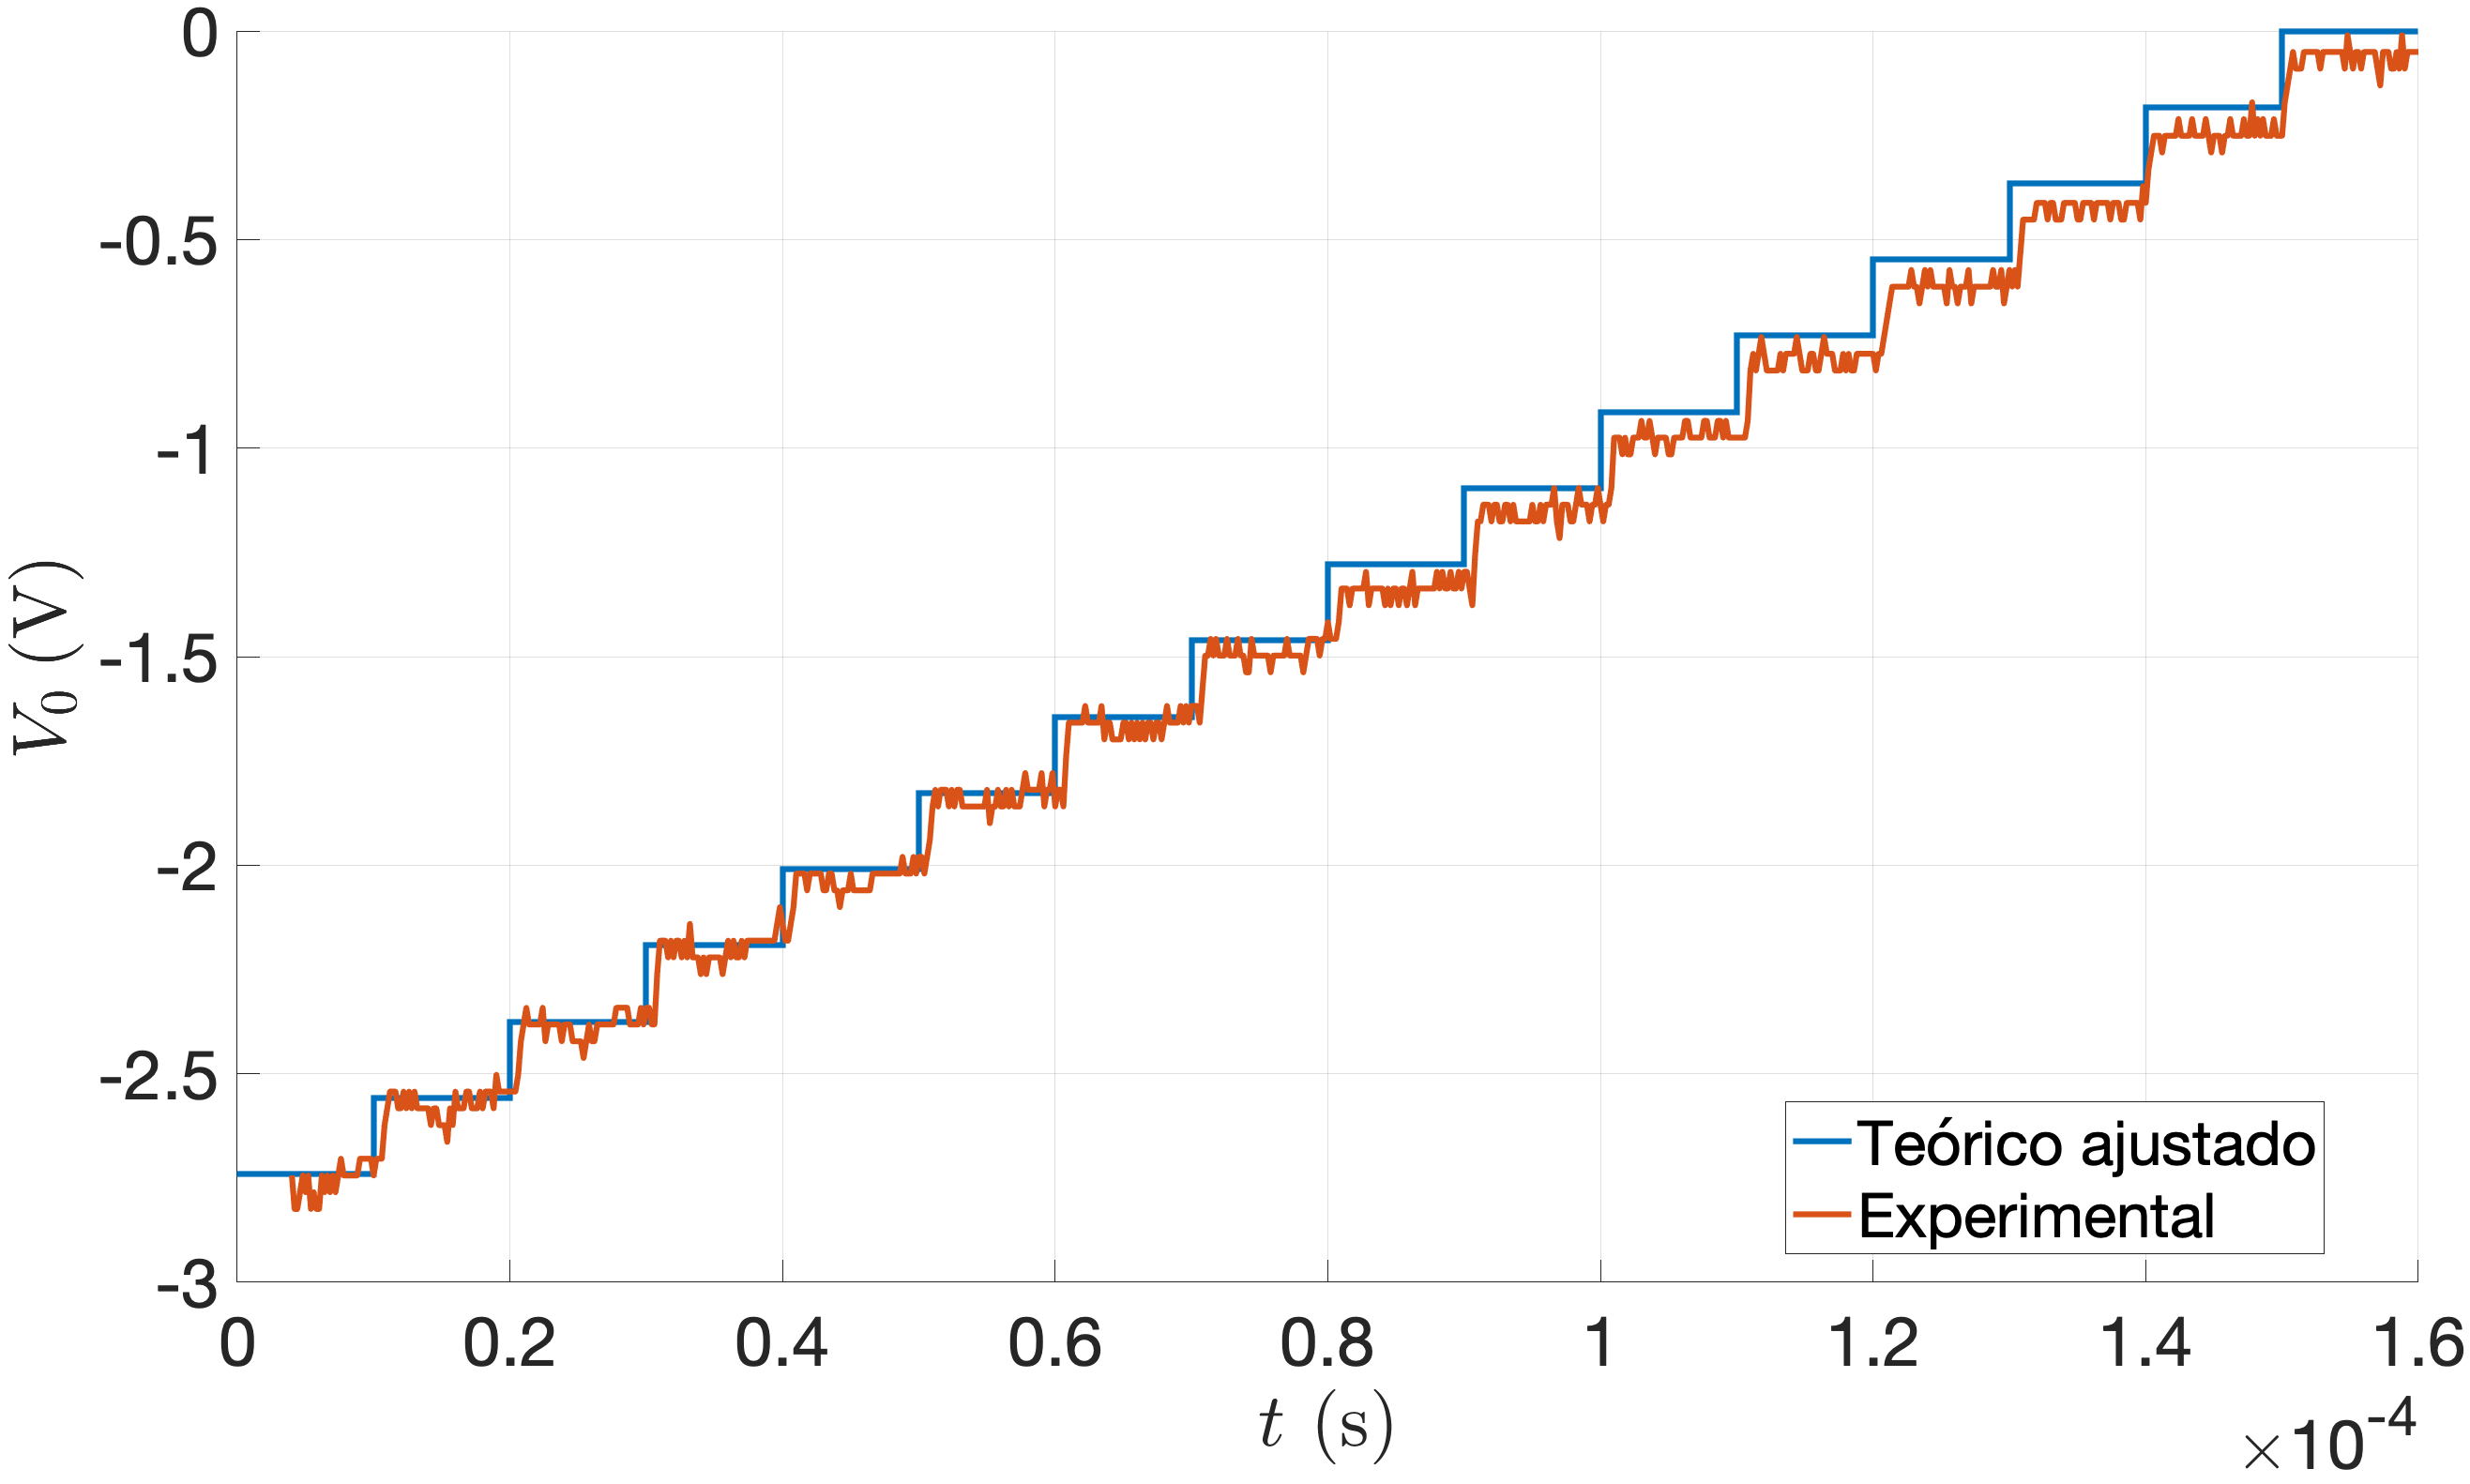
\includegraphics[width=\textwidth]{figures/cteAj_4_3_2_DAC_2R.png}
		\caption{$R_f=2R$.\\}
		\label{fig:cteAj_4_3_2_DAC_2R}
	\end{subfigure}%
	\hfill
	\begin{subfigure}[b]{0.5\textwidth}
		\centering
		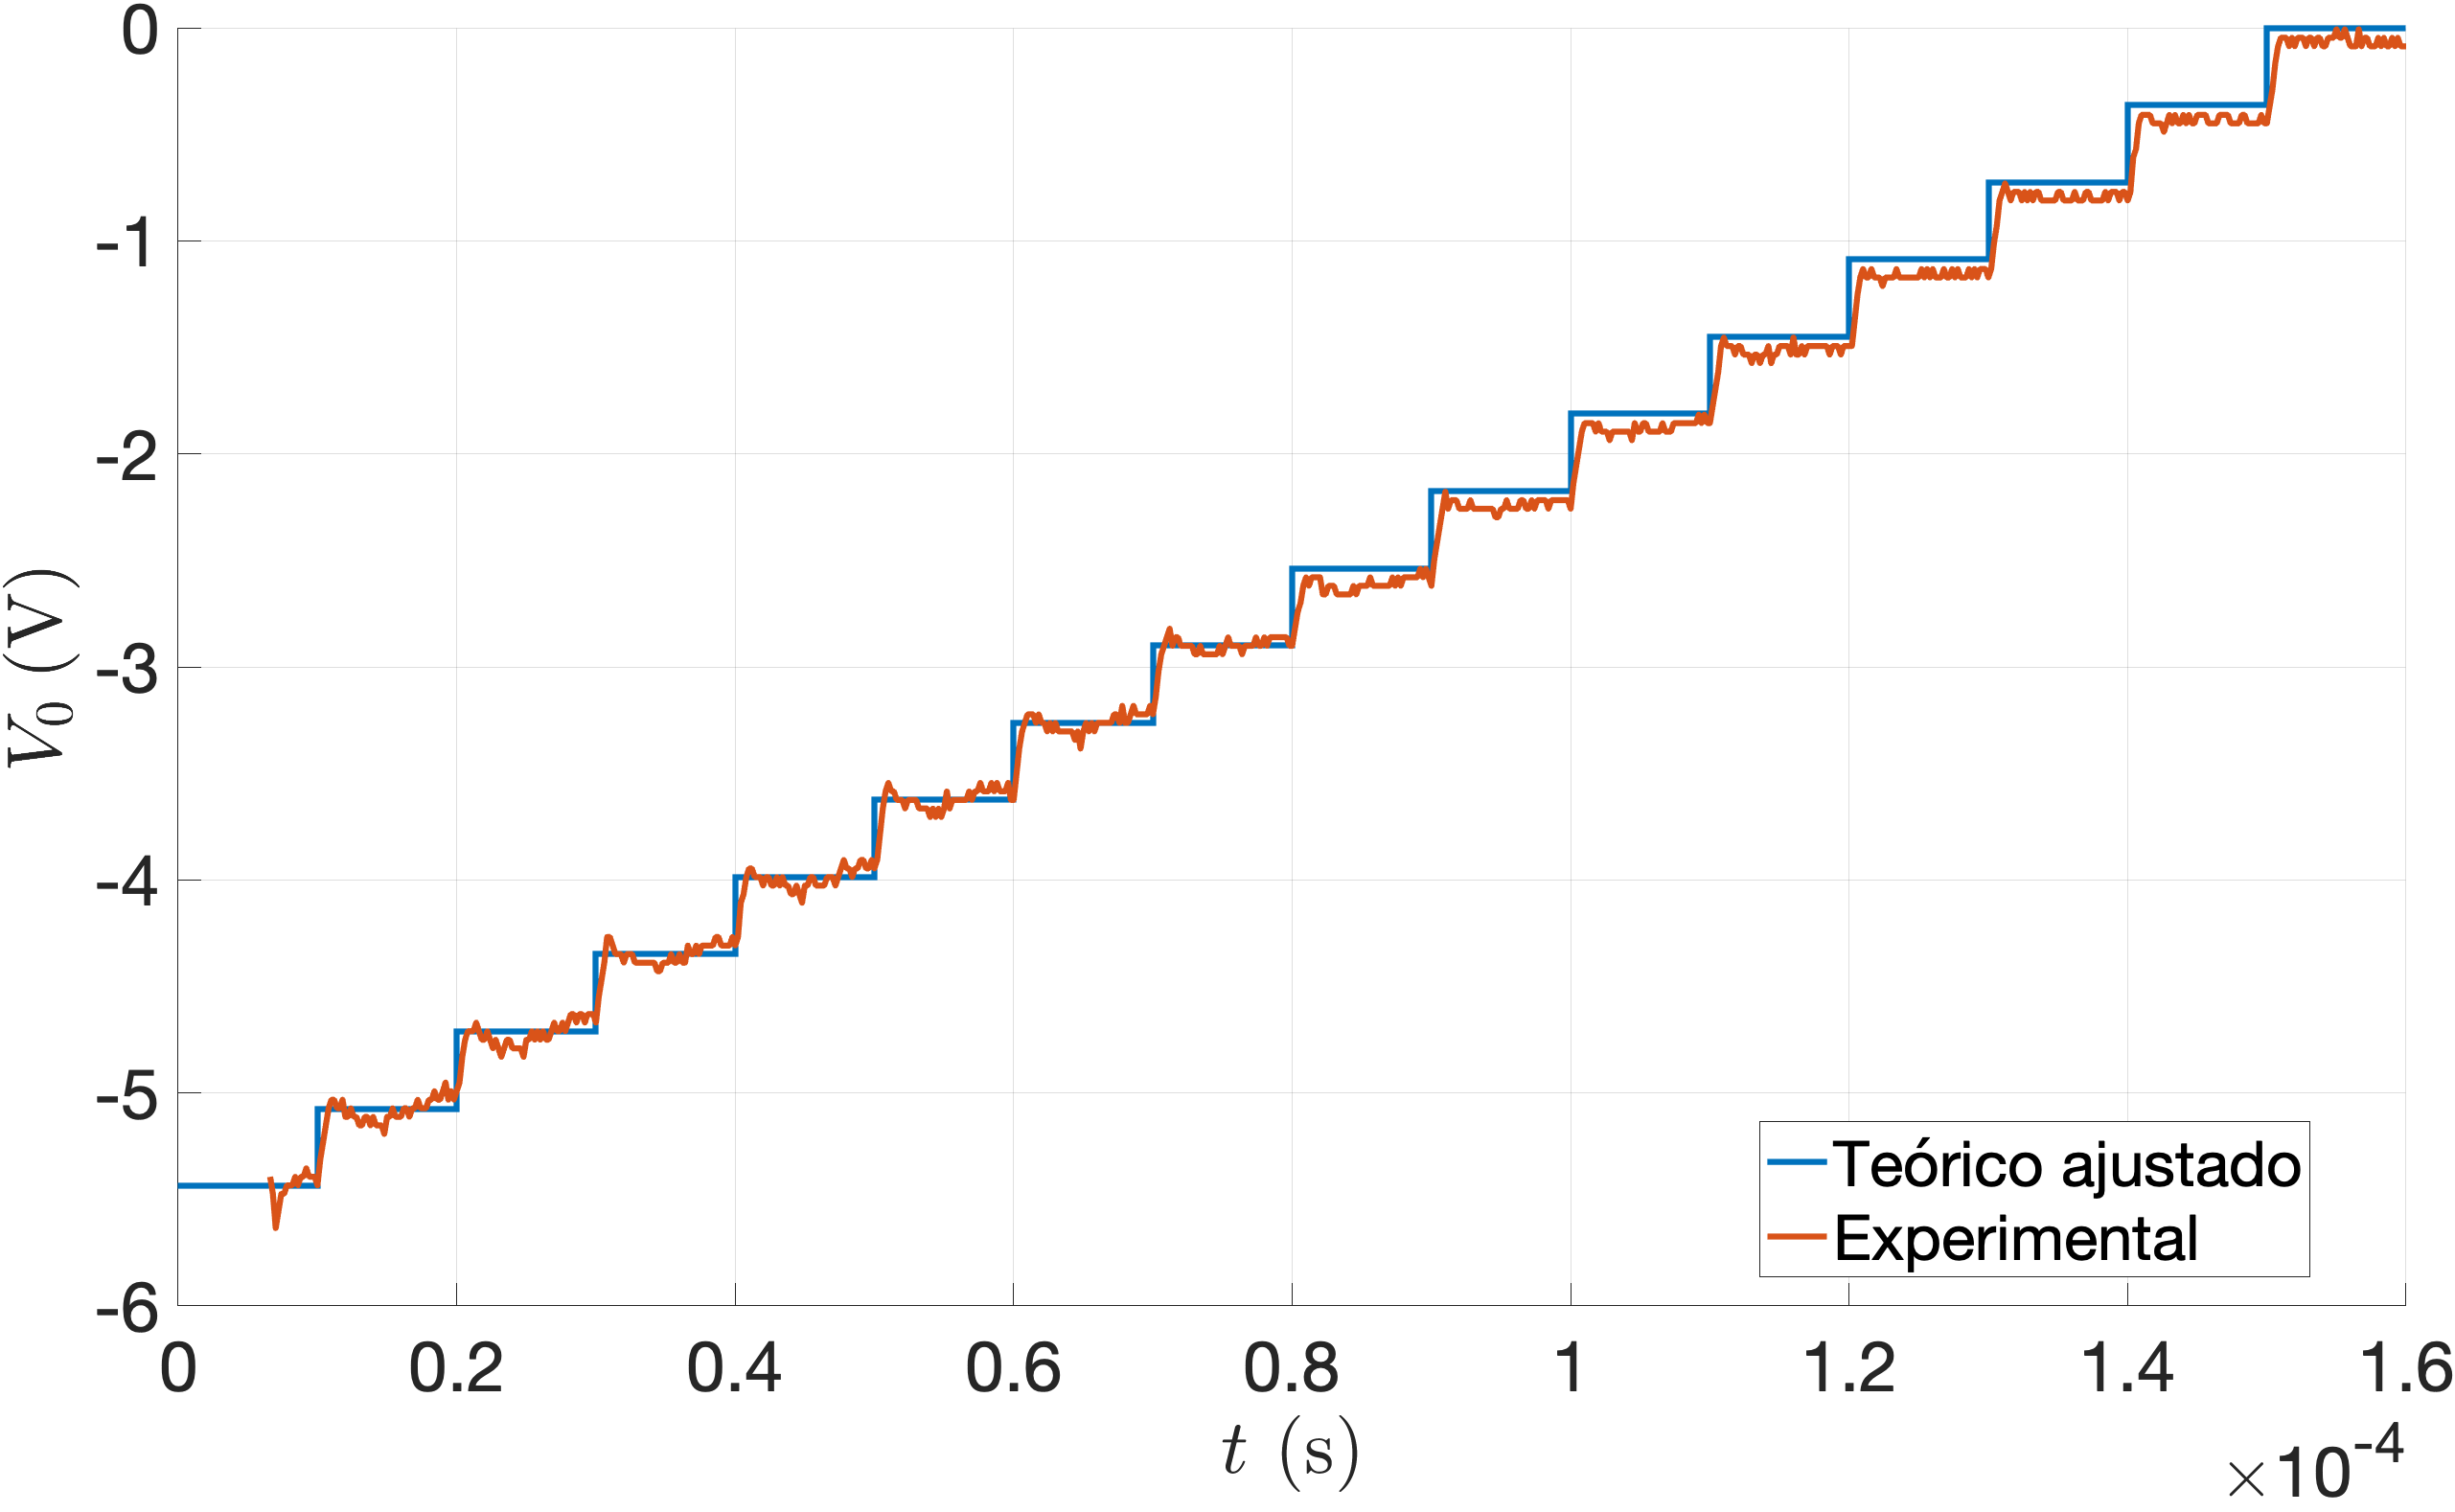
\includegraphics[width=\textwidth]{figures/cteAj_4_3_2_DAC_4R.png}
		\caption{$R_f=4R$.\\}
		\label{fig:cteAj_4_3_2_DAC_4R}
	\end{subfigure}%
	\caption{Comparação dos sinais observados no osciloscópio da saída do DAC com os esperados teoricamente, após ajuste de $V_{ref}$ e $R_f$.\\}
	\label{fig:cteAj_4_3_2_DAC}
\end{figure}


\section{Influência das resistências de entrada}
\subsection{Trabalho experimental}
A montagem da Fig. \ref{fig:esquema_DAC} foi executada  no módulo experimental TEE-08, apresentado na Fig. \ref{sec:modulo_experimental}, de forma a que numa primeira instância $R_1 = 2R$ é substituído por $R$ e numa segunda instância $R_4 = 2R$ é substituído por R. O valor da resistência $R_f$ é mantido a $R_f = 4R$ nos dois ensaios. Na Fig.\ref{fig:DAC_R1_R4_exp} são apresentadas as formas de onda observadas em laboratório para a substituição de $R_1$ e $R_4$ respetivamente. Analisando estas formas de onda verifica-se que a sua forma é muito semelhante ao esperado teoricamente, apresentado graficamente na Fig. \ref{fig:contador_tensao_R1_R4}. Na verdade, é possível distinguir a transição $Q=7\rightarrow Q=8$ aquando da substituição de $R_4$, como sendo a mais expressiva. Para além disso, à semelhança do observado na Secção \ref{sec:estudoFunc} para  também visível que, a transição do patamar de maior tensão para o patamar de menor tensão não é instantânea. Este fenómeno é devido ao \textit{slew rate} do AmpOp e será estudado com mais detalhe na Secção \ref{sec:slewRate}.


\begin{figure}[ht]
	\centering
	\begin{subfigure}[b]{0.5\textwidth}
		\centering
		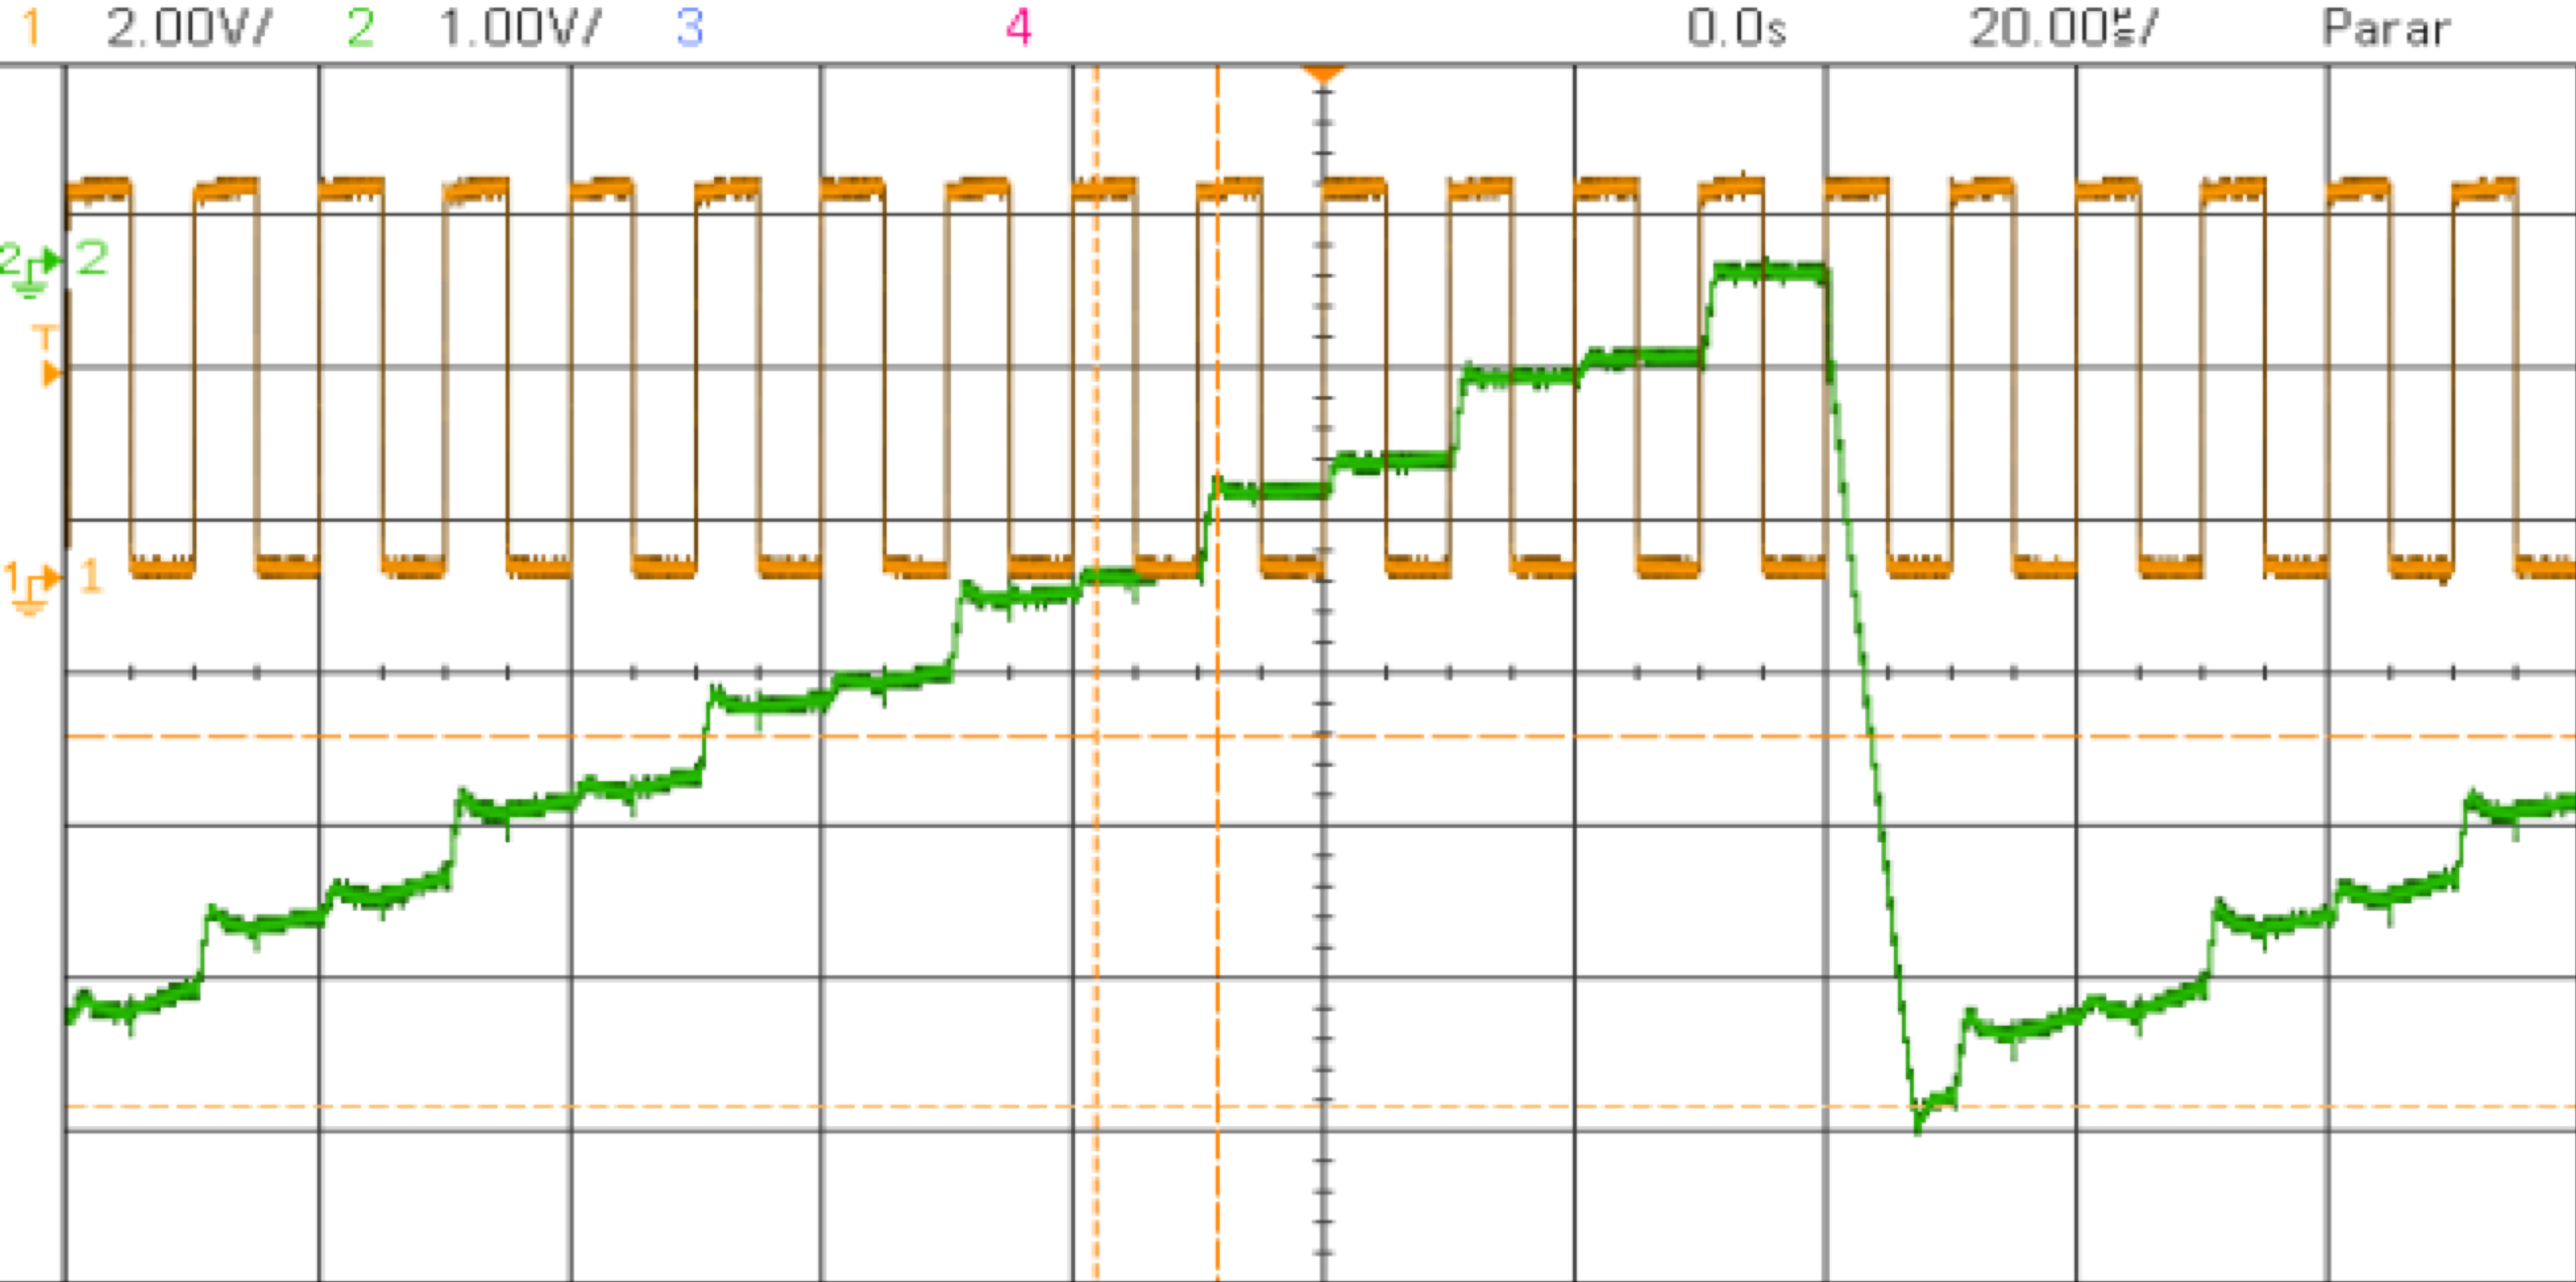
\includegraphics[width=\textwidth]{figures/DAC_R1_exp.png}
		\caption{Substituição de $R_1$.}
		\label{fig:DAC_R1_exp}
	\end{subfigure}%
	\hfill
	\begin{subfigure}[b]{0.5\textwidth}
		\centering
		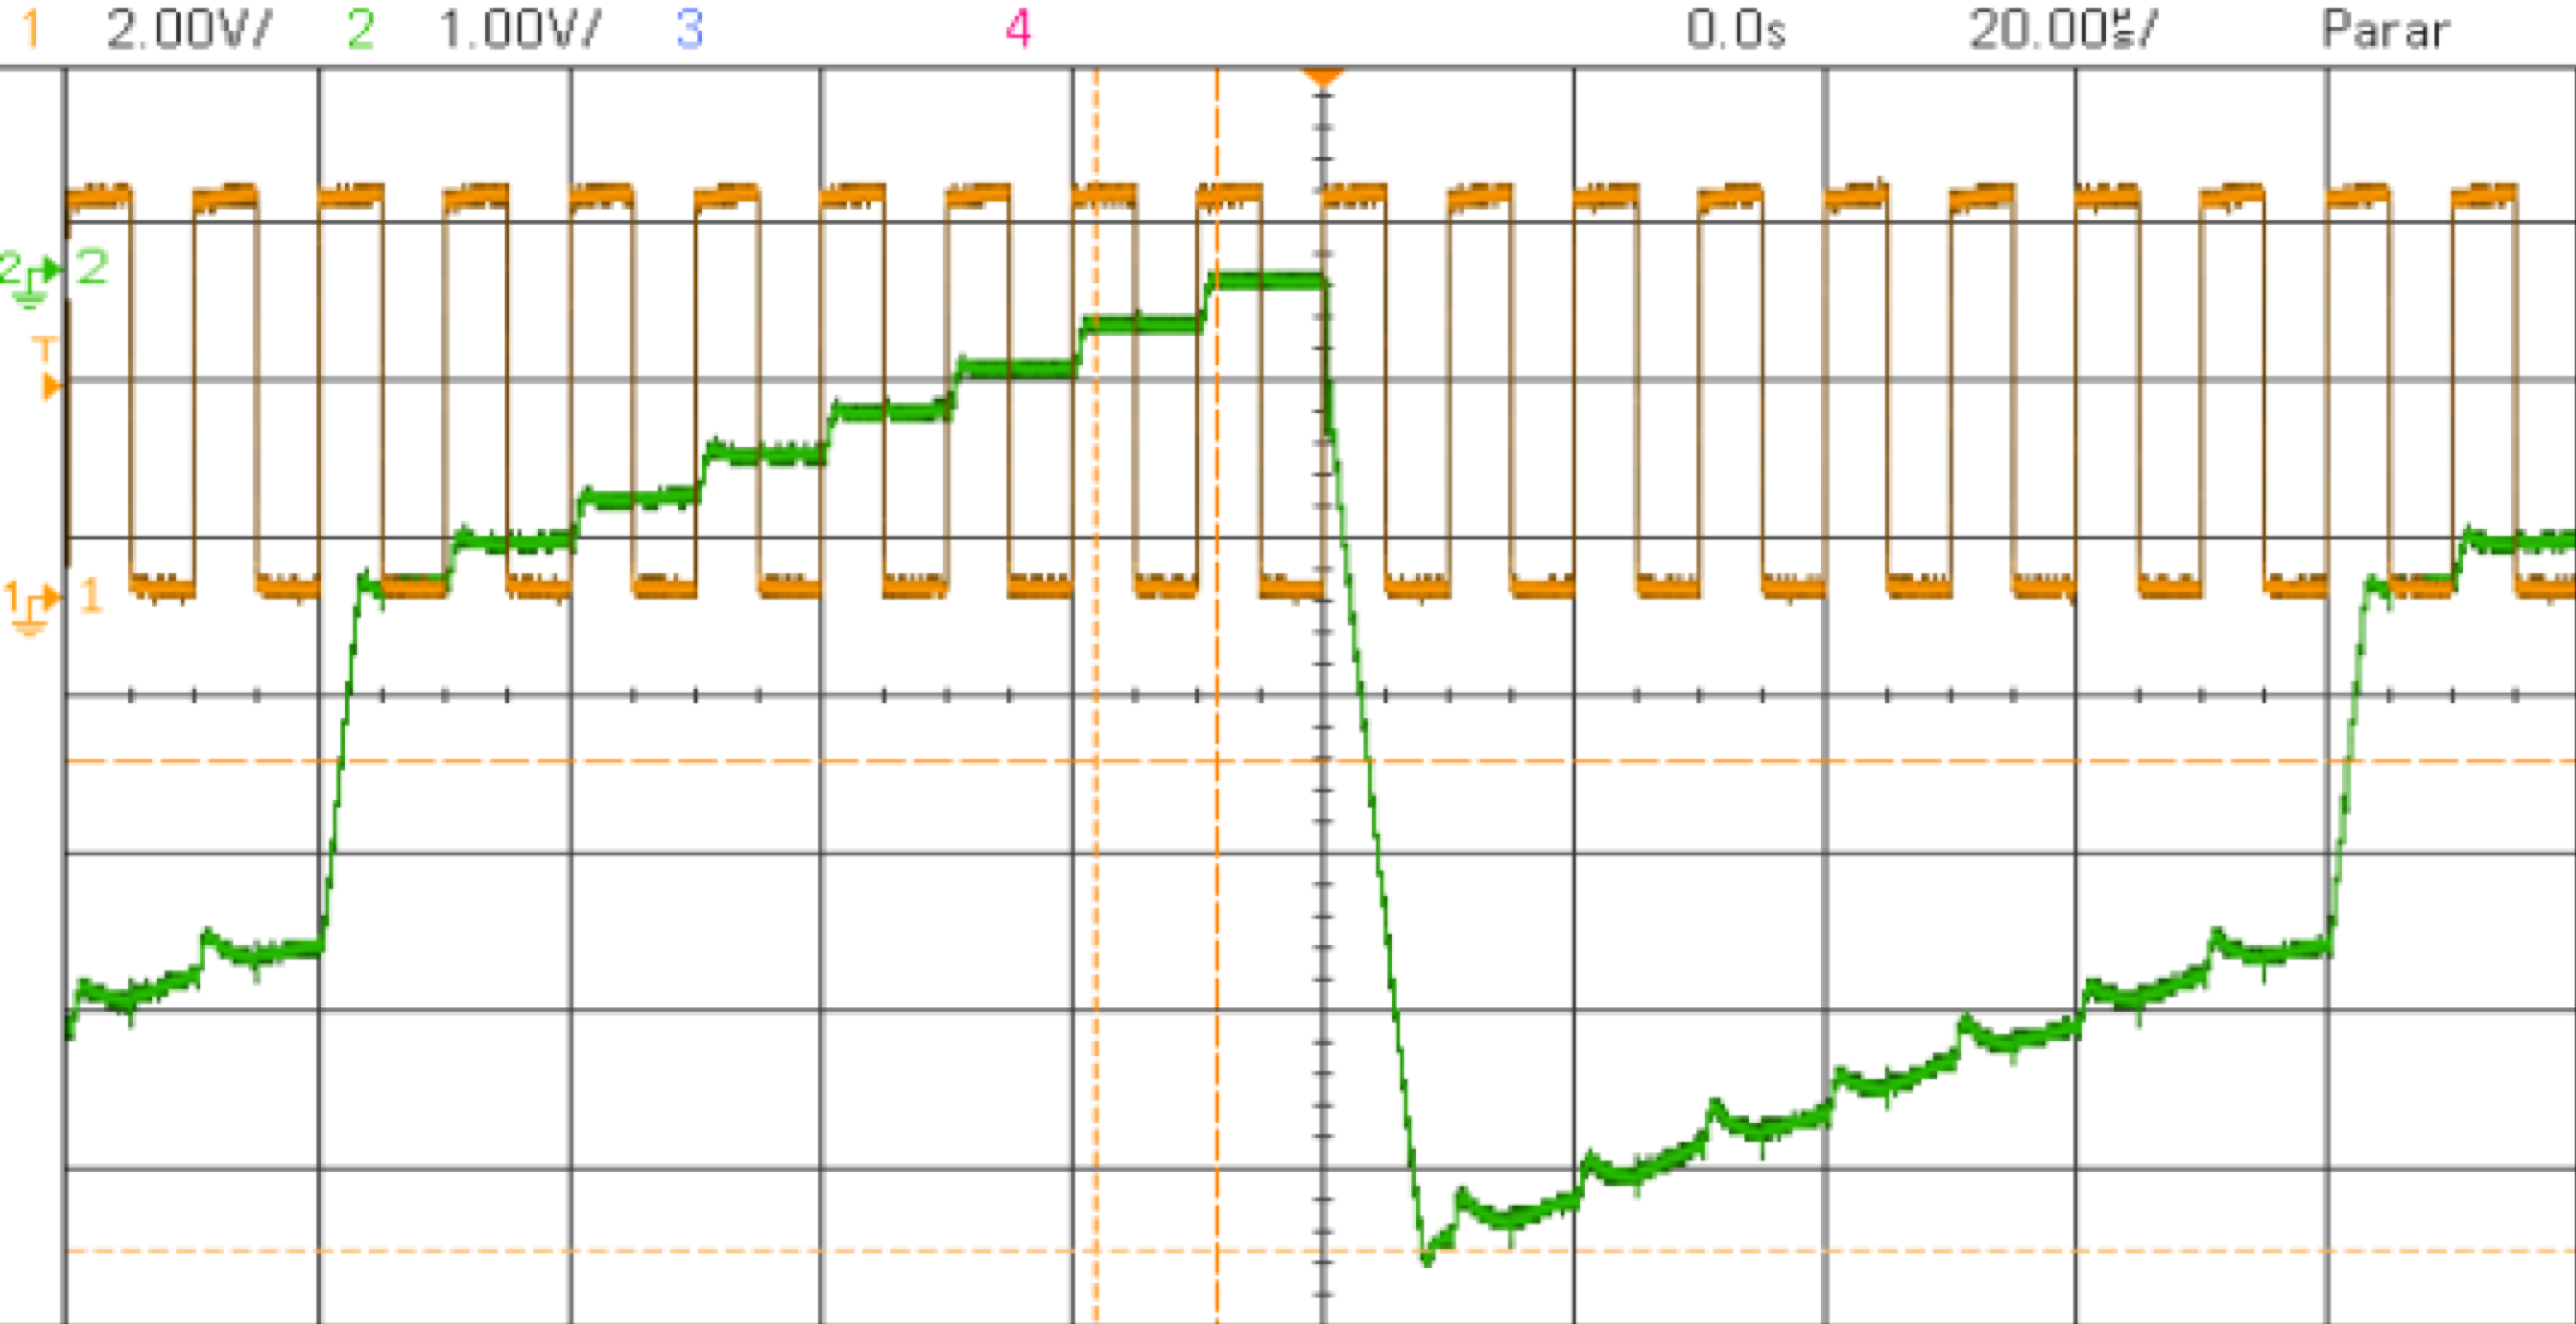
\includegraphics[width=\textwidth]{figures/DAC_R4_exp.png}
		\caption{Substituição de $R_4$.}
		\label{fig:DAC_R4_exp}
	\end{subfigure}%
	\caption{Sinais observados no osciloscópio da saída do DAC (verde) e do sinal de \textit{clock} (laranja).\\}
	\label{fig:DAC_R1_R4_exp}
\end{figure}

\subsection{Comparação de resultados}

Nesta subsecção os resultados experimentais obtidos em laboratório, e apresentados na subsecção anterior, são analisados com detalhe e comparados com os previstos teoricamente na Secção \ref{sec:DAC_R1_R4_teor}. Na Fig. \ref{fig:5_1_2_DAC} são apresentados os sinais observados nos osciloscópio no laboratório com os previstos teoricamente, para 16 períodos de \textit{clock}, tanto para a substituição de $R_1$ como de $R_4$. Foi omitida a transição $15\rightarrow 0$, visto que ela será estudada detalhadamente na Secção \ref{sec:slewRate}. Ao analisar estas figuras, comparando os valores experimentais com os teóricos é evidente, à semelhança dos resultados experimentais da Secção \ref{sec:estudoFunc}  a existência de um grande desfasamento entre eles. Na verdade, verificamos que, para ambas as substituições, a componente principal do desfazamento verificado é proporcional à tensão de saída do DAC, não existindo uma componente de erro não proporcional que seja significativa, corroborando a análise da origem do desfasamento dos resultados experimentais efetuada na Secção \ref{sec:estudoFunc}.

\begin{figure}[ht]
	\centering
	\begin{subfigure}[b]{0.5\textwidth}
		\centering
		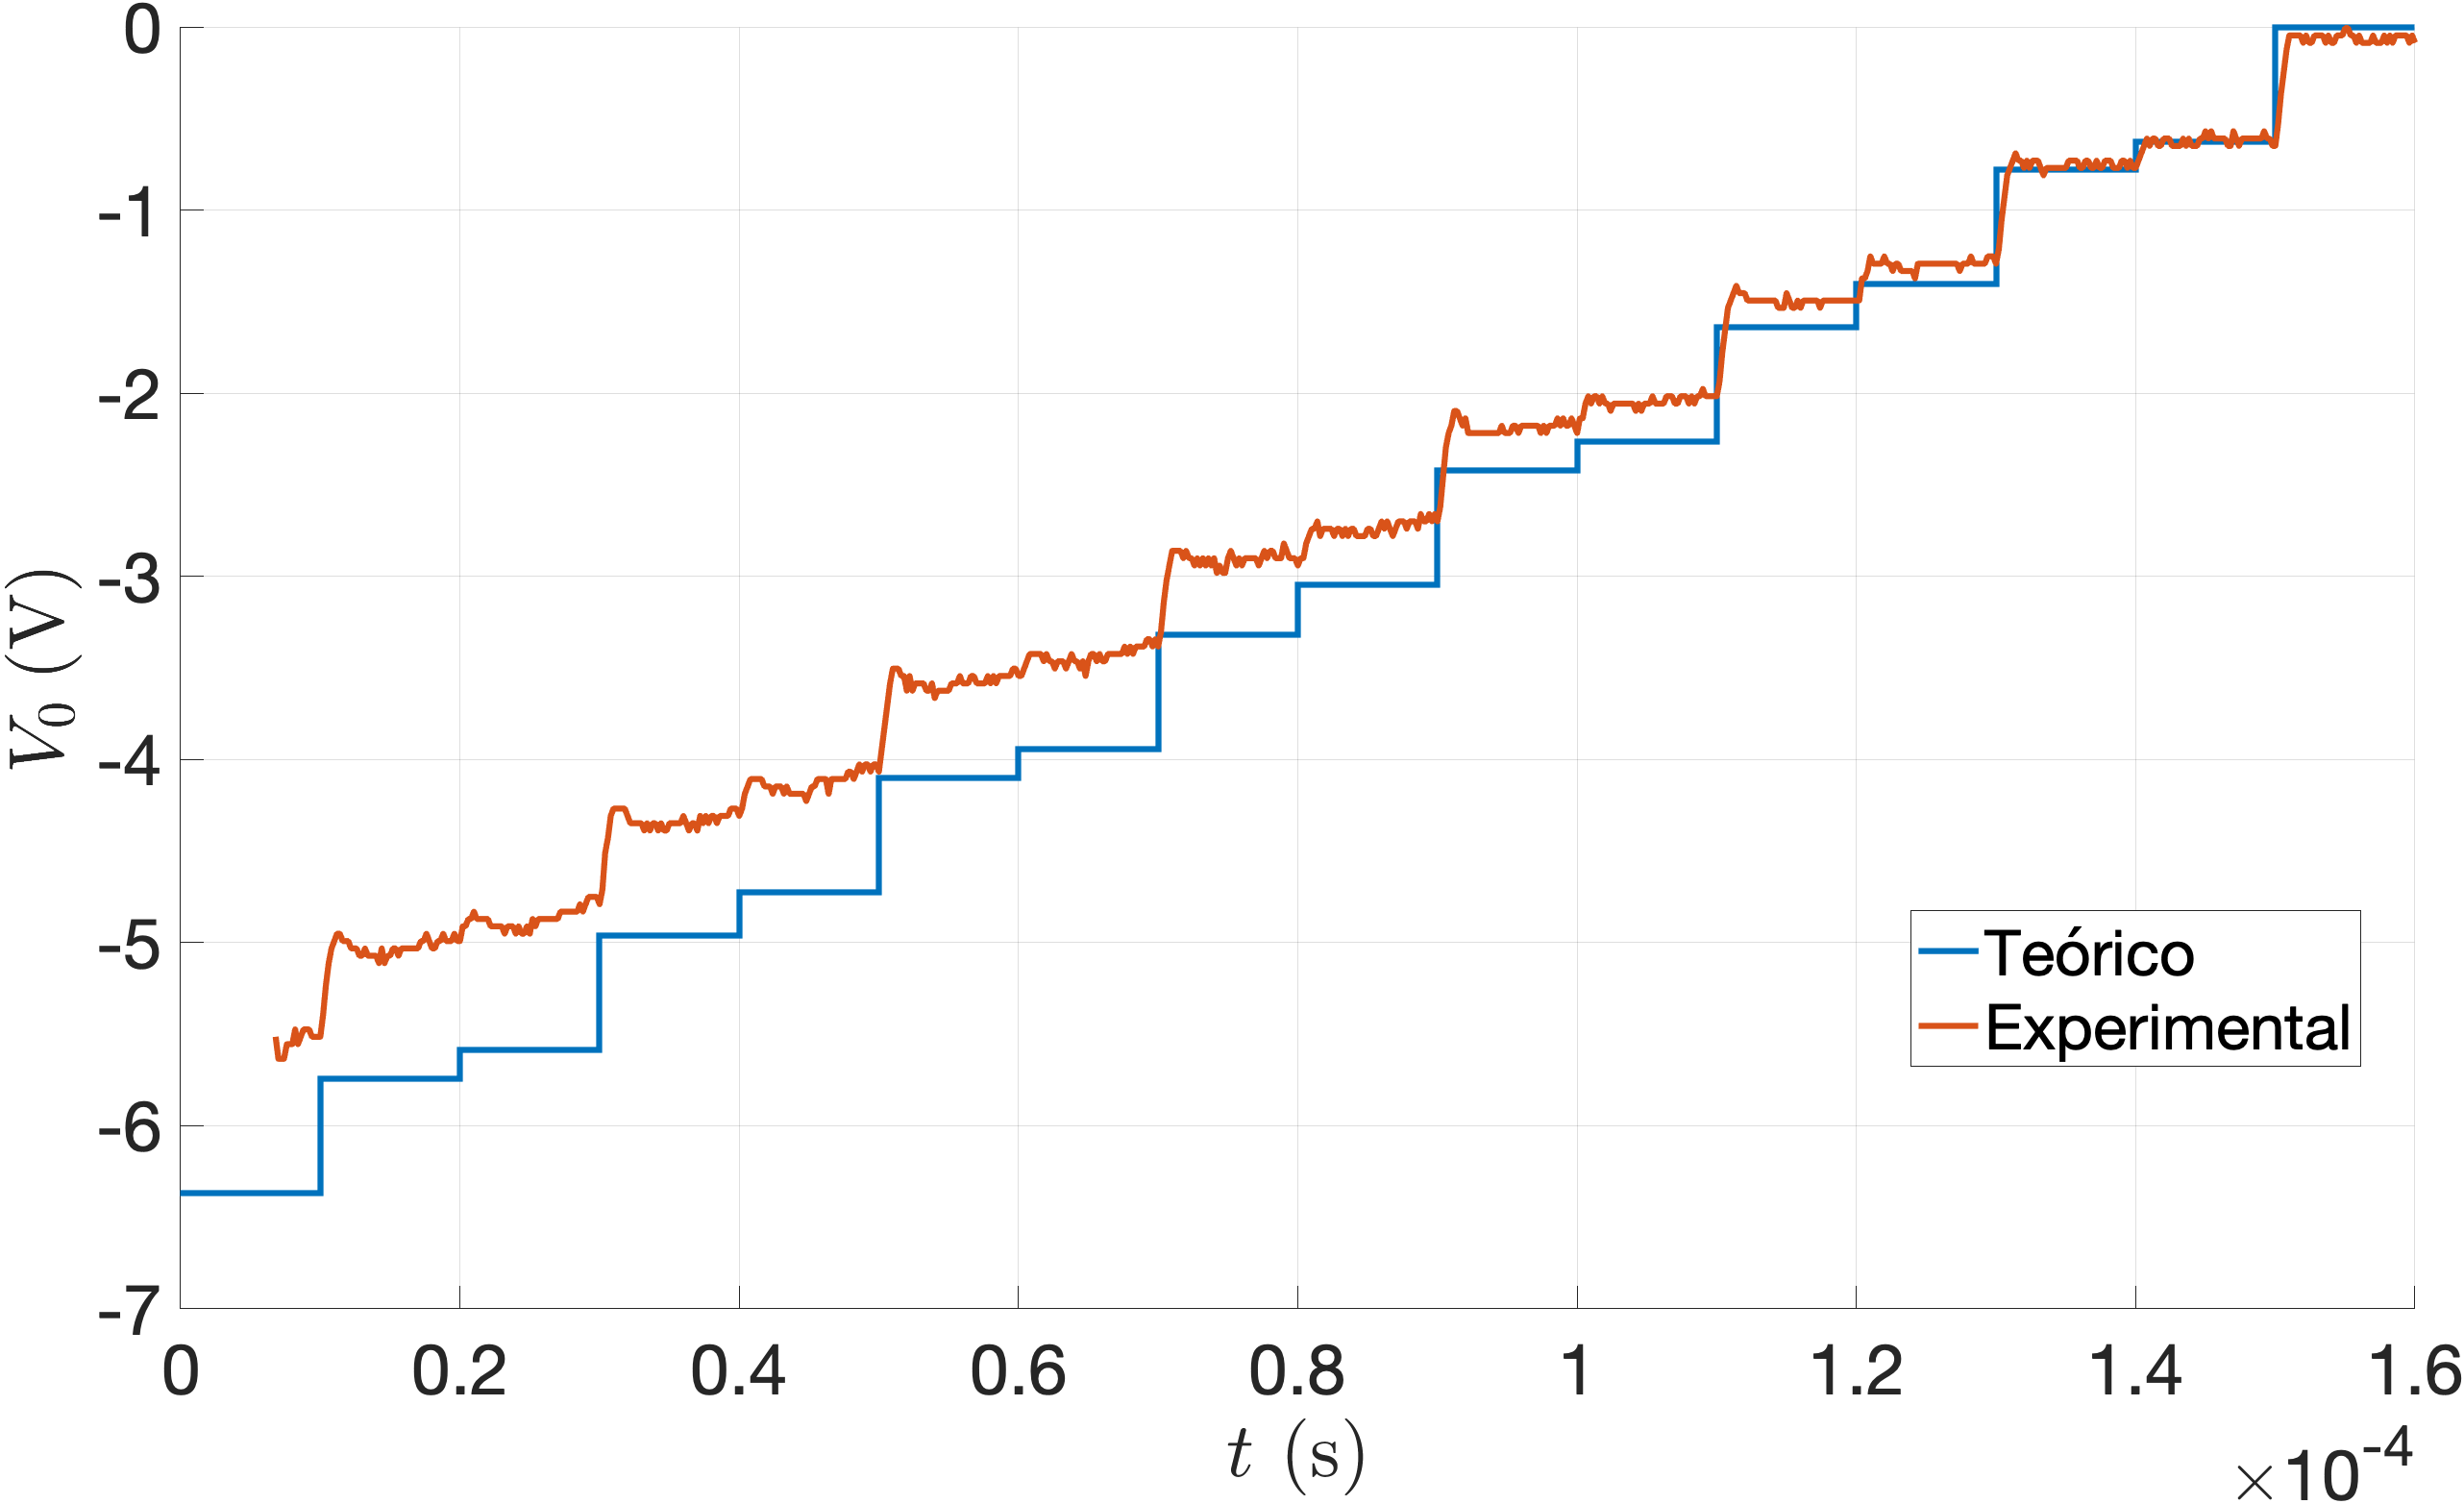
\includegraphics[width=\textwidth]{figures/5_1_2_DAC_R1.png}
		\caption{Substituição de $R_1$.}
		\label{fig:5_1_2_DAC_R1}
	\end{subfigure}%
	\hfill
	\begin{subfigure}[b]{0.5\textwidth}
		\centering
		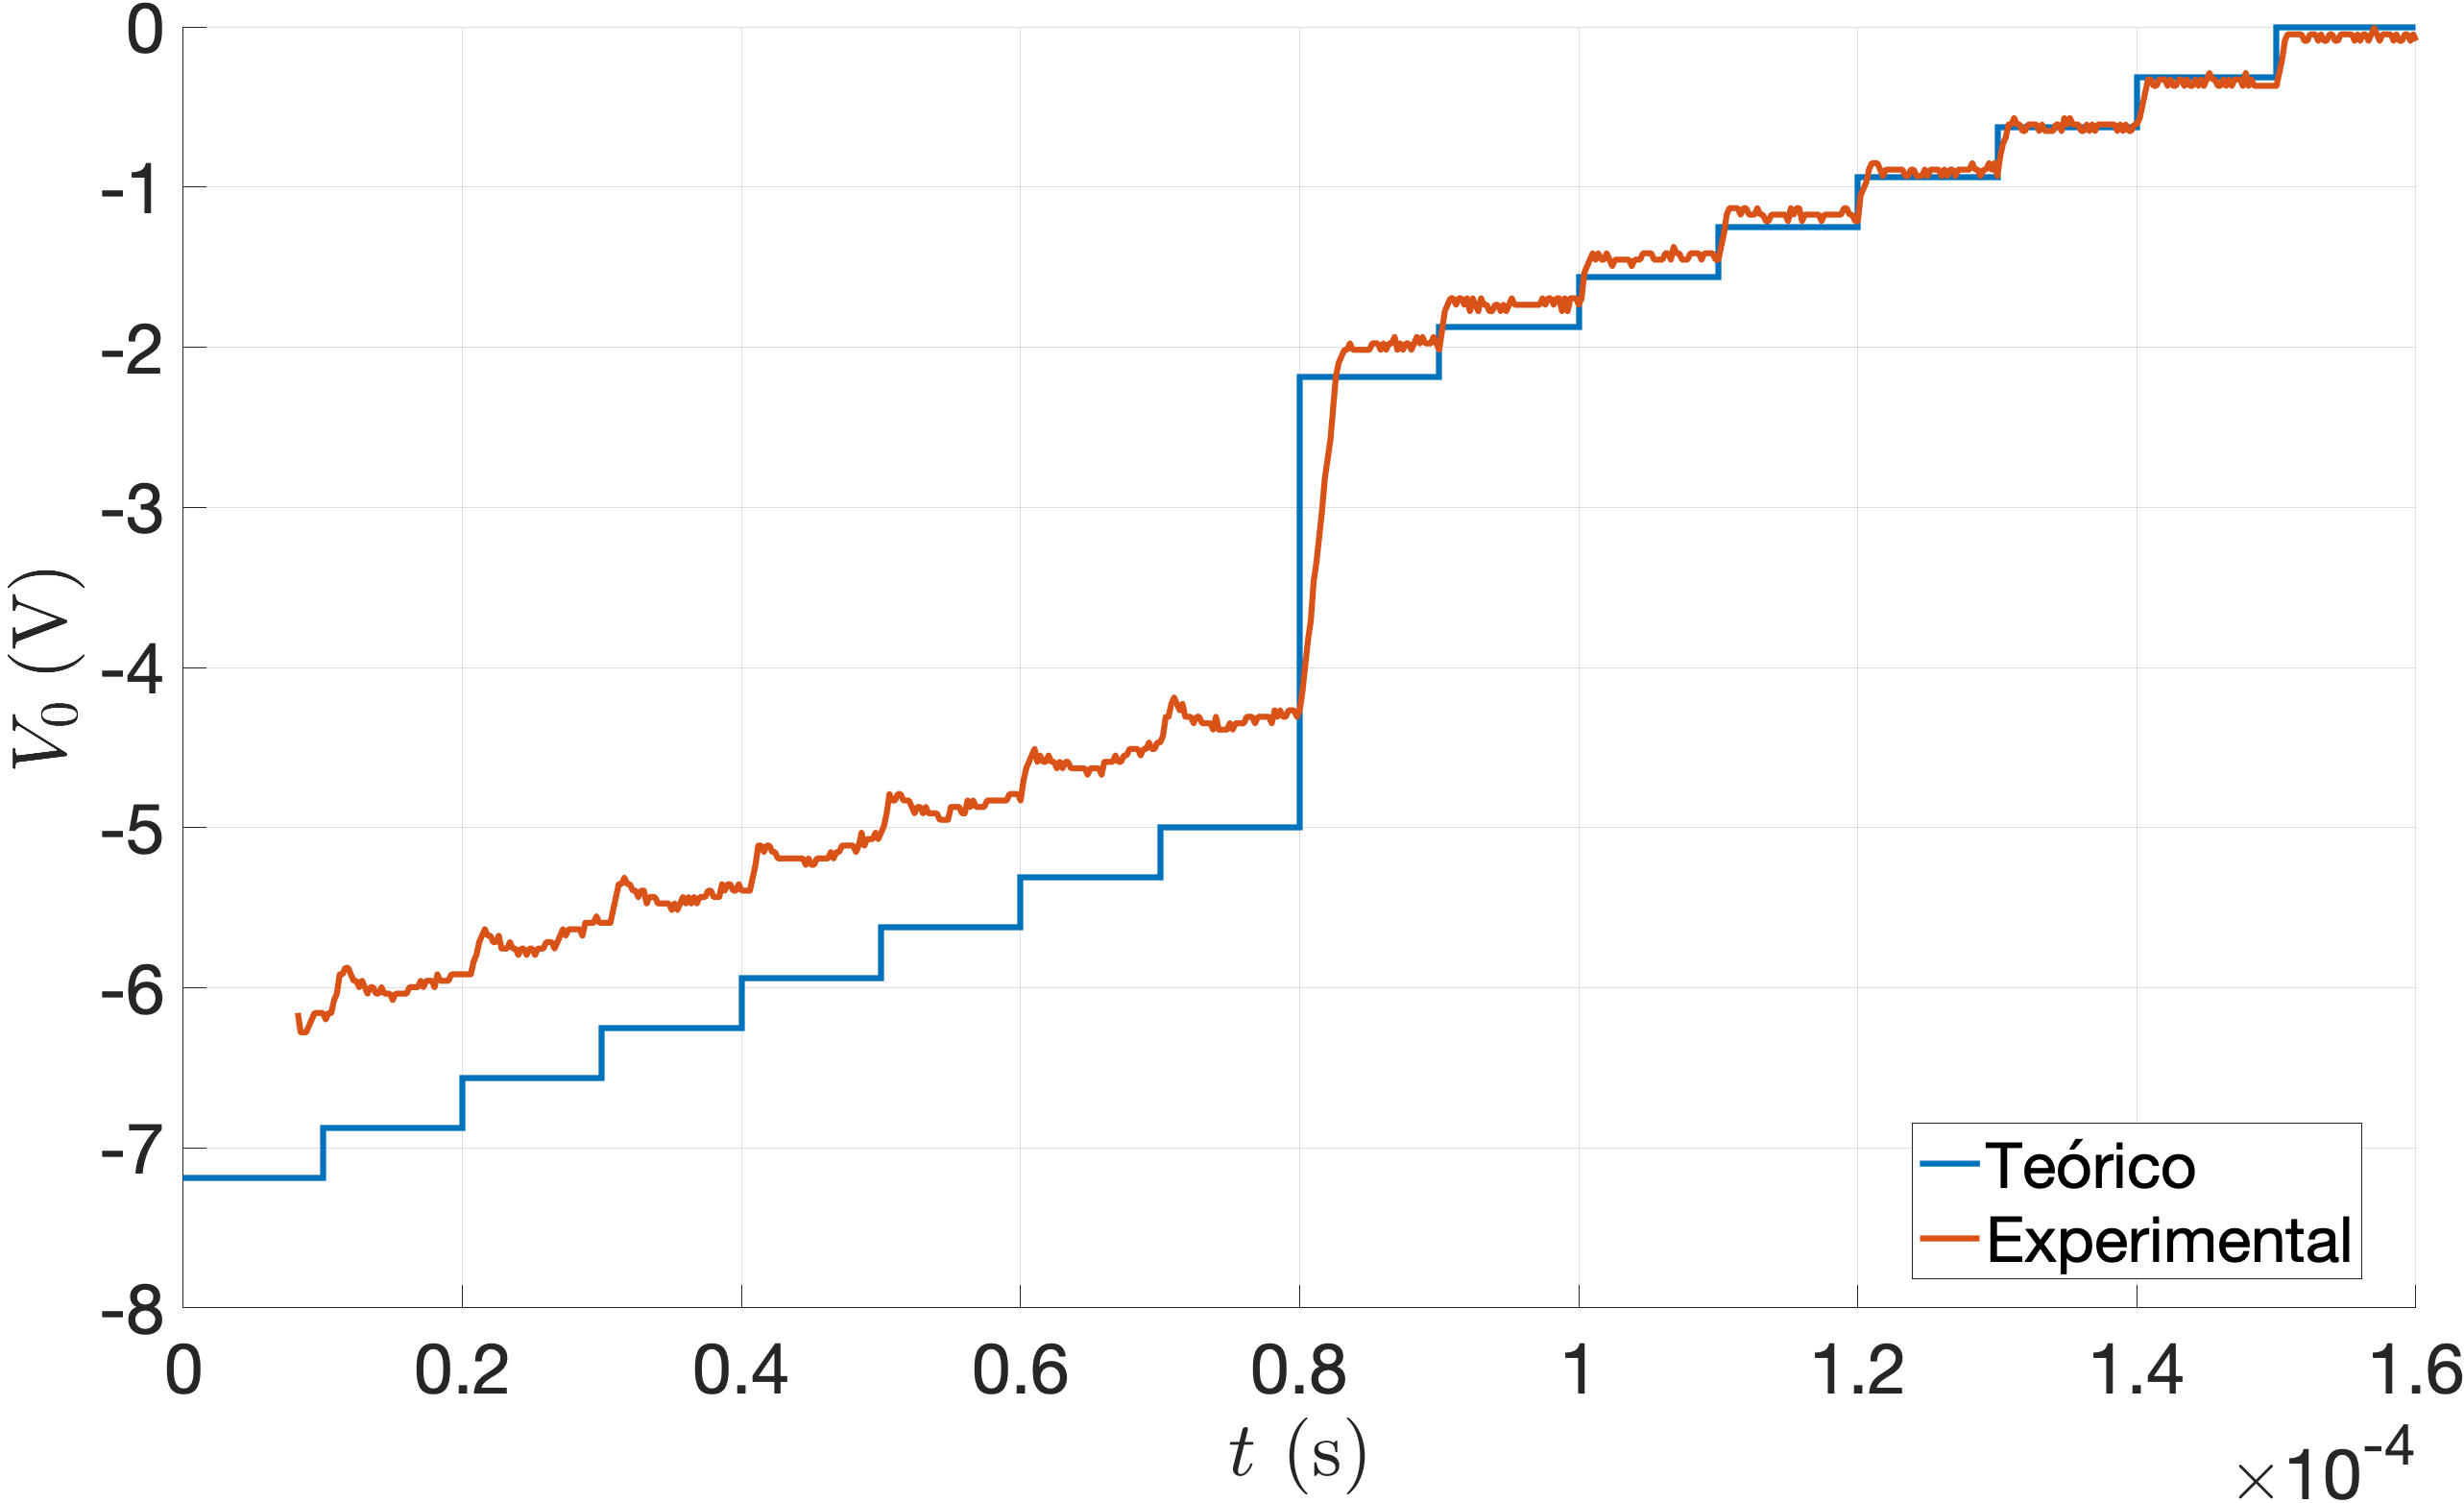
\includegraphics[width=\textwidth]{figures/5_1_2_DAC_R4.png}
		\caption{Substituição de $R_4$.}
		\label{fig:5_1_2_DAC_R4}
	\end{subfigure}%
	\caption{Comparação dos sinais observados no osciloscópio da saída do DAC com os esperados teoricamente, ao longo de 16 períodos de \textit{clock}.\\}
	\label{fig:5_1_2_DAC}
\end{figure}

Por forma avaliar com mais detalhe e objetivamente o desfasamento entre resultados teóricos e experimentais, a determinação do valor dos patamares de tensão experimentais correspondendo a cada um dos números representados em binário à saída das portas lógicas NOR. O procedimento para a determinação da tensão dos patamares é igual ao descrito na Secção \ref{sec:cmpEstudoFunc}.  Os valores de tensão de cada patamar obtidos experimentalmente, bem como a sua comparação com o respetivos valores previstos teoricamente, são apresentados nas Tabelas \ref{tab:Pat_R1_exp} e \ref{tab:Pat_R4_exp}, respetivamente para a substituição de $R_1$ e de $R_4$. Como observado na análise das formas de onda obtidas no laboratório verificamos que para $Q = 0,\ldots,7$, para ambos os valores de $R_f$, o desfazamento relativo é aproximadamente constante, indicando a presença de erro proporcional com a tensão, corroborando a análise da origem do desfasamento dos resultados experimentais efetuada na Secção \ref{sec:estudoFunc}. Para além disso, verifica-se que para valores de $Q>7$ a tensão $V_0$ é mais reduzida em módulo, portanto a componente proporcional do erro deixa de ser preponderante, e outras componentes do erro associadas ao método experimental começam a fazer-se notar, como por exemplo, desfazamentos nos valores das resistências da escada R-2R e o erro de quantização do osciloscópio. É de salientar que o elevado erro relativo visível para $Q=14$ com a substituição de $R_4$ é causados pelo facto de se estar a trabalhar mais reduzidas, e a exatidão das medições nesta situação se degradar. A degradação da exatidão é devida ao baixo rácio sinal-ruído (SNR) num sinal próximo de 0.  

\begin{table}[ht]
	\centering
	\caption{Comparação entre a tensão dos patamares medida experimentalmente e esperada teoricamente para a substituição de $R_1$.}
	\label{tab:Pat_R1_exp}
	\begin{tabular}{ccccc}
		$Q$ & Teórico (V) & Experimental (V) & Erro absoluto (V) & Erro relativo\\
		\hline
		0 & -6.367 & -5.562 & 0.8049 & 12.64\%\\ 
		1 & -5.742 & -5.056 & 0.6864 & 11.95\%\\ 
		2 & -5.586 & -4.905 & 0.6809 & 12.19\%\\ 
		3 & -4.961 & -4.358 & 0.6026 & 12.15\%\\ 
		4 & -4.727 & -4.157 & 0.5693 & 12.04\%\\ 
		5 & -4.102 & -3.596 & 0.5051 & 12.31\%\\ 
		6 & -3.945 & -3.458 & 0.4875 & 12.36\%\\ 
		7 & -3.320 & -2.923 & 0.3972 & 11.96\%\\ 
		8 & -3.047 & -2.754 & 0.2926 & 9.603\%\\ 
		9 & -2.422 & -2.202 & 0.2204 & 9.099\%\\ 
		10 & -2.266 & -2.053 & 0.2129 & 9.395\%\\ 
		11 & -1.641 & -1.504 & 0.1366 & 8.326\%\\ 
		12 & -1.406 & -1.307 & 0.09922 & 7.055\%\\ 
		13 & -0.7812 & -0.7583 & 0.02296 & 2.939\%\\ 
		14 & -0.6250 & -0.6216 & 0.003392 & 0.5428\%\\ 
		15 & 0.0000 & -0.05879 & -0.05879 & -- \\
		\hline
	\end{tabular}
\end{table}


\begin{table}[ht]
	\centering
	\caption{Comparação entre a tensão dos patamares medida experimentalmente e esperada teoricamente para a substituição de $R_4$.}
	\label{tab:Pat_R4_exp}
	\begin{tabular}{ccccc}
		$Q$ & Teórico (V) & Experimental (V) & Erro absoluto (V) & Erro relativo\\
		\hline
		0 & -7.188 & -6.206 & 0.9820 & 13.66\%\\ 
		1 & -6.875 & -6.023 & 0.8524 & 12.40\%\\ 
		2 & -6.562 & -5.751 & 0.8112 & 12.36\%\\ 
		3 & -6.250 & -5.462 & 0.7882 & 12.61\%\\ 
		4 & -5.938 & -5.194 & 0.7430 & 12.51\%\\ 
		5 & -5.625 & -4.897 & 0.7280 & 12.94\%\\ 
		6 & -5.312 & -4.618 & 0.6949 & 13.08\%\\ 
		7 & -5.000 & -4.352 & 0.6477 & 12.95\%\\ 
		8 & -2.188 & -2.001 & 0.1870 & 8.548\%\\ 
		9 & -1.875 & -1.739 & 0.1358 & 7.243\%\\ 
		10 & -1.562 & -1.44 & 0.1228 & 7.859\%\\ 
		11 & -1.250 & -1.174 & 0.07563 & 6.050\%\\ 
		12 & -0.9375 & -0.907 & 0.03047 & 3.250\%\\ 
		13 & -0.6250 & -0.6236 & 0.001382 & 0.2212\%\\ 
		14 & -0.3125 & -0.3442 & -0.03172 & -10.15\%\\ 
		15 & 0.0000 & -0.06281 & -0.06281 & --\\
	
		\hline
	\end{tabular}
\end{table}

Na Fig. \ref{fig:cteAj_5_1_2_DAC} são apresentados os sinais observados nos osciloscópio com os previstos teoricamente com os parâmetros $R_f$ e $V_{ref}$ ajustados, para 16 períodos de \textit{clock}, tanto para a substituição de $R_1$ como de $R_4$. Os valores de tensão de cada patamar obtidos experimentalmente, bem como a sua comparação com o respetivos valores teóricos ajustados, são apresentados nas Tabelas \ref{tab:Pat_R1_exp_Aj} e \ref{tab:Pat_R4_exp_Aj}, respetivamente para a substituição de $R_1$ e de $R_4$. Verificamos que, de facto, os valores previstos teoricamente calculados com os parâmetros ajustados são muito próximos dos observados no laboratório. Este resultados laboratoriais não foram usados para o ajuste dos parâmetros, pelo que podemos afirmar, dado o bom modelo do DAC com $R_f$ e $V_{ref}$ ajustados, que é esta a fonte predominante de erro verificada nos resultados laboratoriais das Secções \ref{sec:infRes} e \ref{sec:estudoFunc}. É visível, no entanto, que ainda existe uma componente de erro sistemático para $Q>7$, obtendo-se resultados experimentais consistentemente inferiores aos previsão teórica ajustada. Este desfazamento deve-se a desvios em relação aos valores nominais da escada R-2R, que foram desprezados no cálculo de da previsão teórica ajustada. Para além disso, para tensões baixas em módulo à saída do DAC, o sinal amostrado tem um baixo SNR, pelo que é esperado que os erros relativos aumentem à medida que a saída de aproxima de 0.

\begin{figure}[ht]
	\centering
	\begin{subfigure}[b]{0.5\textwidth}
		\centering
		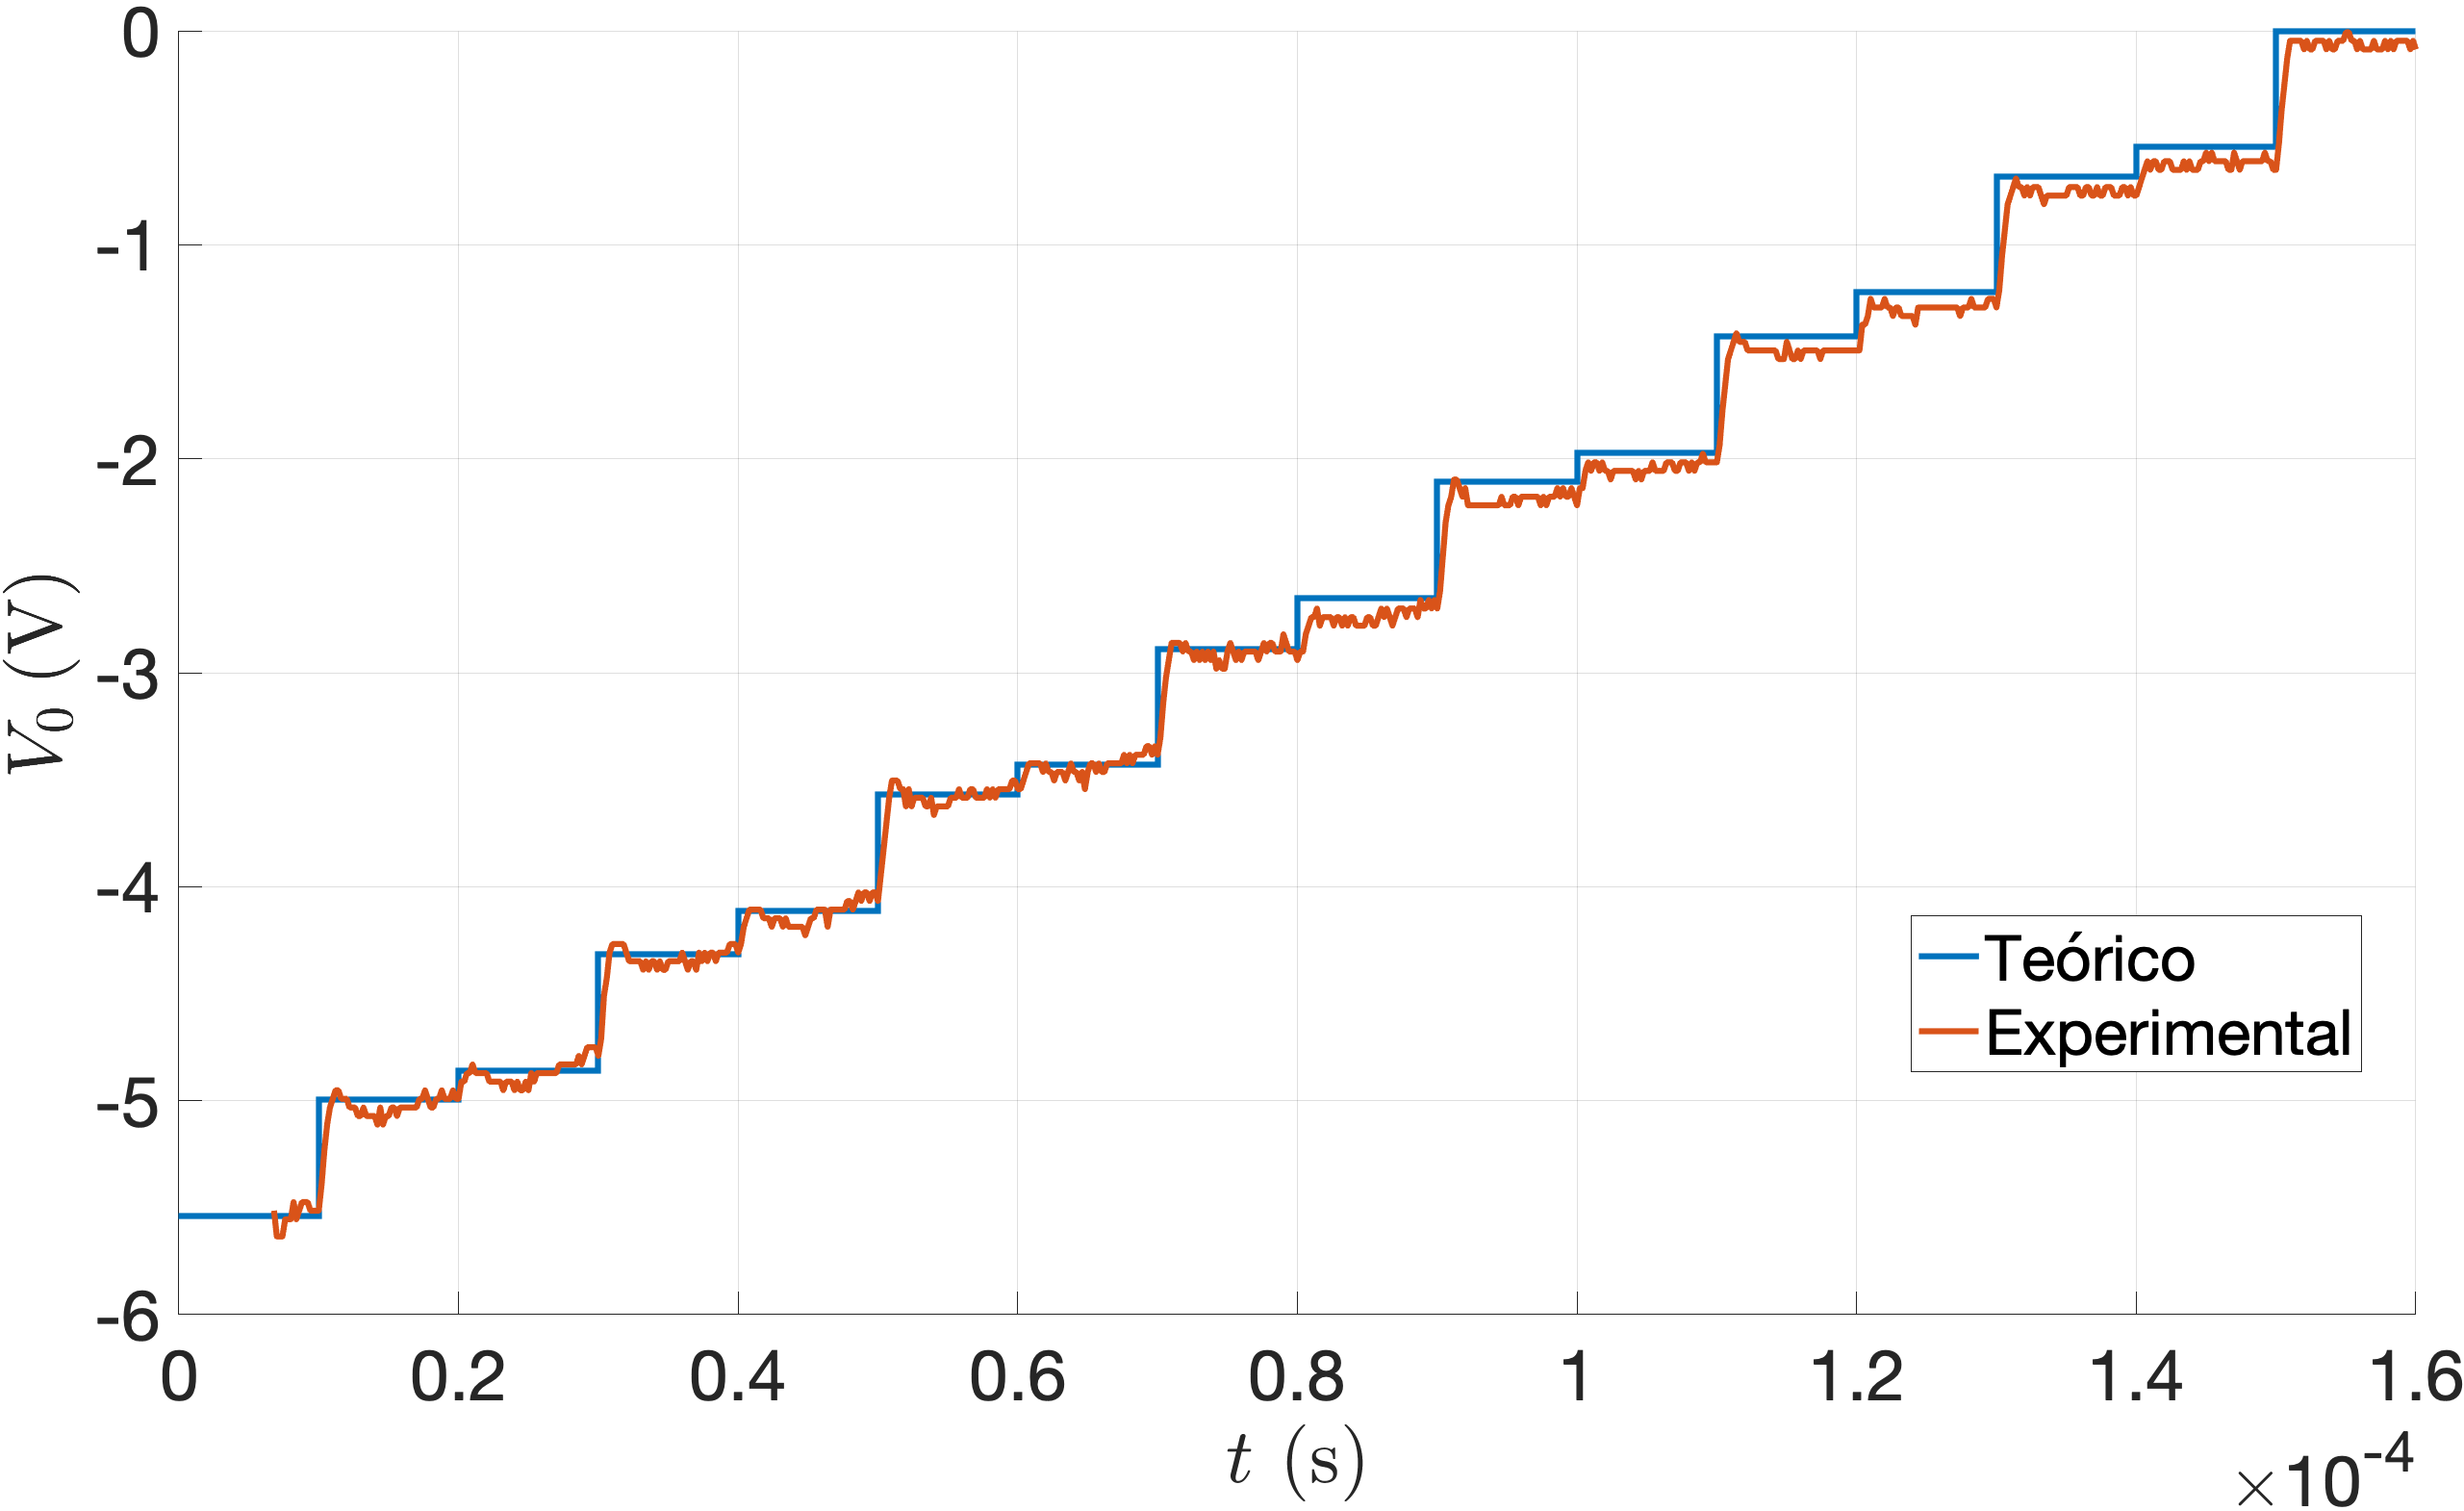
\includegraphics[width=\textwidth]{figures/cteAj_5_1_2_DAC_R1.png}
		\caption{Substituição de $R_1$.}
		\label{fig:cteAj_5_1_2_DAC_R1}
	\end{subfigure}%
	\hfill
	\begin{subfigure}[b]{0.5\textwidth}
		\centering
		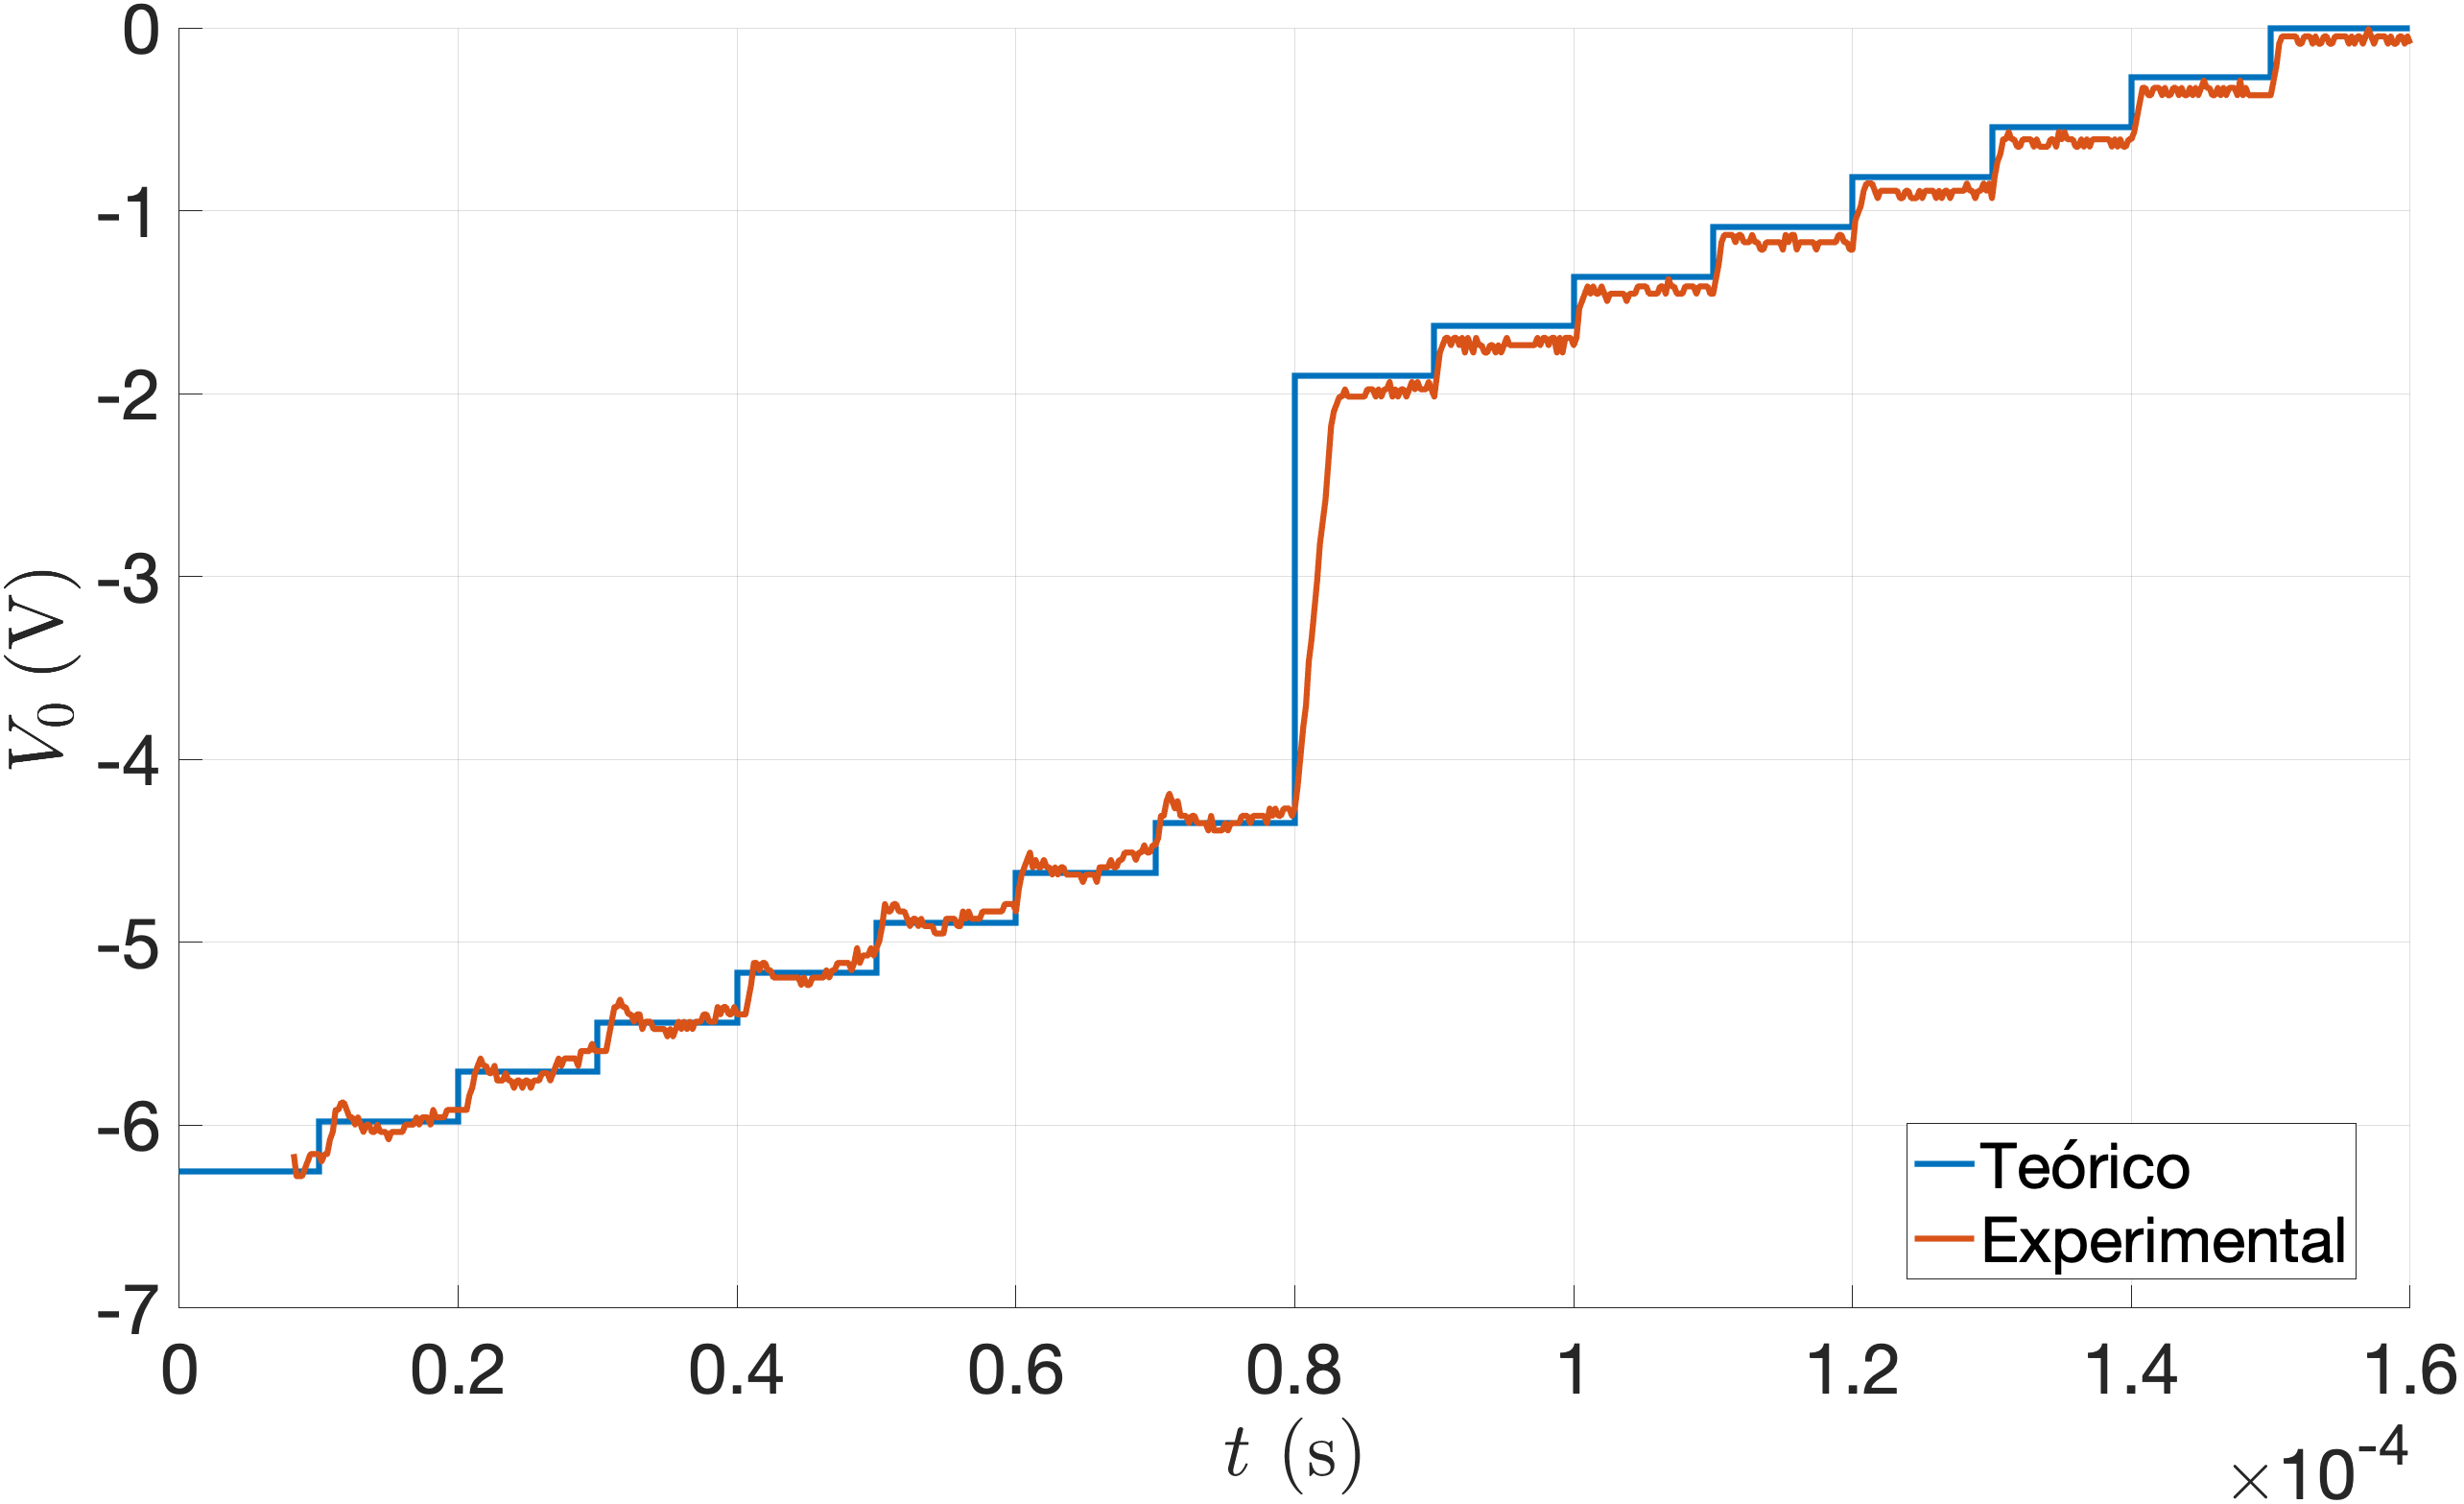
\includegraphics[width=\textwidth]{figures/cteAj_5_1_2_DAC_R4.png}
		\caption{Substituição de $R_4$.}
		\label{fig:cteAj_5_1_2_DAC_R4}
	\end{subfigure}%
	\caption{Comparação dos sinais observados no osciloscópio da saída do DAC com os esperados teoricamente, após ajuste de $V_{ref}$ e $R_f$.}
	\label{fig:cteAj_5_1_2_DAC}
\end{figure}

\begin{table}[ht]
	\centering
	\caption{Comparação entre a tensão dos patamares medida experimentalmente e esperada teoricamente para a substituição de $R_1$, após ajuste de $V_{ref}$ e $R_f$.}
	\label{tab:Pat_R1_exp_Aj}
	\begin{tabular}{ccccc}
		$Q$ & Teórico (V) & Experimental (V) & Erro absoluto (V) & Erro relativo\\
		\hline
		0 & -5.538 & -5.562 & -0.02393 & -0.4322\%\\ 
		1 & -4.995 & -5.056 & -0.06105 & -1.222\%\\ 
		2 & -4.859 & -4.905 & -0.0462 & -0.9509\%\\ 
		3 & -4.315 & -4.358 & -0.04311 & -0.9991\%\\ 
		4 & -4.111 & -4.157 & -0.04598 & -1.118\%\\ 
		5 & -3.568 & -3.596 & -0.02882 & -0.8077\%\\ 
		6 & -3.432 & -3.458 & -0.02603 & -0.7586\%\\ 
		7 & -2.888 & -2.923 & -0.03500 & -1.212\%\\ 
		8 & -2.650 & -2.754 & -0.1040 & -3.924\%\\ 
		9 & -2.107 & -2.202 & -0.09489 & -4.504\%\\ 
		10 & -1.971 & -2.053 & -0.08205 & -4.164\%\\ 
		11 & -1.427 & -1.504 & -0.07695 & -5.392\%\\ 
		12 & -1.223 & -1.307 & -0.08384 & -6.854\%\\ 
		13 & -0.6796 & -0.7583 & -0.07874 & -11.59\%\\ 
		14 & -0.5436 & -0.6216 & -0.07796 & -14.34\%\\ 
		15 & 0.000 & -0.05879 & -0.05879 & --\\
	

		\hline
	\end{tabular}
\end{table}


\begin{table}[ht]
	\centering
	\caption{Comparação entre a tensão dos patamares medida experimentalmente e esperada teoricamente para a substituição de $R_4$, após ajuste de $V_{ref}$ e $R_f$.}
	\label{tab:Pat_R4_exp_Aj}
	\begin{tabular}{ccccc}
		$Q$ & Teórico (V) & Experimental (V) & Erro absoluto (V) & Erro relativo\\
		\hline
		0 & -6.252 & -6.206 & 0.04638 & 0.7419\%\\ 
		1 & -5.980 & -6.023 & -0.04253 & -0.7111\%\\ 
		2 & -5.708 & -5.751 & -0.04299 & -0.7531\%\\ 
		3 & -5.436 & -5.462 & -0.02537 & -0.4666\%\\ 
		4 & -5.165 & -5.194 & -0.02985 & -0.5780\%\\ 
		5 & -4.893 & -4.897 & -0.004186 & -0.08555\%\\ 
		6 & -4.621 & -4.618 & 0.003389 & 0.07334\%\\ 
		7 & -4.349 & -4.352 & -0.003107 & -0.07143\%\\ 
		8 & -1.903 & -2.001 & -0.09775 & -5.137\%\\ 
		9 & -1.631 & -1.739 & -0.1083 & -6.638\%\\ 
		10 & -1.359 & -1.440 & -0.08059 & -5.929\%\\ 
		11 & -1.087 & -1.174 & -0.08708 & -8.009\%\\ 
		12 & -0.8155 & -0.9070 & -0.09157 & -11.23\%\\ 
		13 & -0.5436 & -0.6236 & -0.07997 & -14.71\%\\ 
		14 & -0.2718 & -0.3442 & -0.07240 & -26.63\%\\ 
		15 & 0.0000 & -0.06281 & -0.06281 & --\\
	
		
		\hline
	\end{tabular}
\end{table}


%\begin{table}[h]
%	\centering
%	\caption{Comparação entre diferença entre a tensão em patamares consecutivos medida experimentalmente e esperada teoricamente para a substituição de $R_1$.}
%	\label{tab:difPat_R1_exp}
%	\begin{tabular}{cccc}
%		Transição & Teórico & Experimental & Erro relativo \\
%		\hline
%		$0\rightarrow1$ & 0.6250 & 0.5065 & -18.95\\ 
%		$1\rightarrow2$ & 0.1562 & 0.1508 & -3.518\\
%		$2\rightarrow3$ & 0.6250 & 0.5467 & -12.52\\ 
%		$3\rightarrow4$ & 0.2344 & 0.2010 & -14.24\\ 
%		$4\rightarrow5$ & 0.6250 & 0.5608 & -10.27\\ 
%		$5\rightarrow6$ & 0.1562 & 0.1387 & -11.24\\
%		$6\rightarrow7$ & 0.6250 & 0.5347 & -14.45\\ 
%		$7\rightarrow8$ & 0.2734 & 0.1688 & -38.25\\ 
%		$8\rightarrow9$ & 0.6250 & 0.5528 & -11.56\\ 
%		$9\rightarrow10$ & 0.1562 & 0.1487 & -4.804\\ 
%		$10\rightarrow11$ & 0.6250 & 0.5487 & -12.20\\ 
%		$11\rightarrow12$ & 0.2344 & 0.1970 & -15.95\\
%		$12\rightarrow13$ & 0.625 & 0.5487 & -12.20\\ 
%		$13\rightarrow14$0 & 0.1562 & 0.1367 & -12.52\\ 
%		$14\rightarrow15$ & 0.6250 & 0.5628 & -9.950\\
%		\hline
%	\end{tabular}
%\end{table}
%
%\begin{table}[h]
%	\centering
%	\caption{Comparação entre diferença entre a tensão em patamares consecutivos medida experimentalmente e esperada teoricamente para a substituição de $R_1$.}
%	\label{tab:difPat_R1_exp}
%	\begin{tabular}{cccc}
%		Transição & Teórico & Experimental & Erro relativo \\
%		\hline
%		$0\rightarrow1$ & 0.6250 & 0.5065 & -18.95\\ 
%		$1\rightarrow2$ & 0.1562 & 0.1508 & -3.518\\
%		$2\rightarrow3$ & 0.6250 & 0.5467 & -12.52\\ 
%		$3\rightarrow4$ & 0.2344 & 0.2010 & -14.24\\ 
%		$4\rightarrow5$ & 0.6250 & 0.5608 & -10.27\\ 
%		$5\rightarrow6$ & 0.1562 & 0.1387 & -11.24\\
%		$6\rightarrow7$ & 0.6250 & 0.5347 & -14.45\\ 
%		$7\rightarrow8$ & 0.2734 & 0.1688 & -38.25\\ 
%		$8\rightarrow9$ & 0.6250 & 0.5528 & -11.56\\ 
%		$9\rightarrow10$ & 0.1562 & 0.1487 & -4.804\\ 
%		$10\rightarrow11$ & 0.6250 & 0.5487 & -12.20\\ 
%		$11\rightarrow12$ & 0.2344 & 0.1970 & -15.95\\
%		$12\rightarrow13$ & 0.625 & 0.5487 & -12.20\\ 
%		$13\rightarrow14$0 & 0.1562 & 0.1367 & -12.52\\ 
%		$14\rightarrow15$ & 0.6250 & 0.5628 & -9.950\\
%		\hline
%	\end{tabular}
%\end{table}

\end{document}
